\chapter{The Interaction of Light with Plasma}%
\label{chap:Theory}

This chapter shall introduce theoretical background relevant to the work conducted in this thesis.
The main focus of the work is centred on improving the laser modelling in the \textsc{Chimera} \ac{Rad-MHD} code.
Therefore, the theoretical framework for modelling both the plasma and the propagation and absorption of light in it is introduced.

To begin, the plasma state is defined and important length- and time-scales are provided in Sec.~\ref{sec:theory_plasma_phys}.
The kinetic and fluid descriptions of plasma are introduced in Sec.~\ref{sec:theory_kin_fluid_plasmas} and the validity domain of each framework is discussed, with particular reference to typical conditions for laser-plasma interactions.
Additional physics packages of the fluid code, \textsc{Chimera}, which are utilised in later chapters, are introduced.
A model for kinetic heatflow is desirable in fluid codes which model laser-plasma interactions.
Therefore, although \textsc{Chimera} does not have this capability, some basic theory of kinetic heatflow modelling is highlighted.

An additional aim of the work was to include a \ac{CBET} model into the new \textsc{Chimera} laser package.
\ac{LPIs} such as \ac{CBET} are multi-wave coupling phenomena, and therefore a basic description of waves in plasma is provided in Sec.~\ref{sec:theory_waves_plasmas}.
The dispersion relation of the light waves in plasma is also derived.
Beginning with the full wave equation and then introducing successive assumptions which are broadly satisfied in typical laser-produced \ac{ICF} plasmas, Sec.~\ref{sec:theory_propagation} derives the equations of ray-tracing.
Important absorption processes are then outlined, particularly \ac{Inv-Brem}, which is the dominant mechanism on the largest \ac{ICF} facilities in the world today.
Finally, the basic theory of \ac{LPIs} is provided in Sec.~\ref{sec:theory_LPIs}, particularly \ac{CBET} and its relevance for direct-drive \ac{ICF}.

\newpage

%###############################################################################################################################
%###############################################################################################################################
%###############################################################################################################################
\section{Basic Plasma Physics}%
\label{sec:theory_plasma_phys}

As stated in Chap.~\ref{chap:intro}, thermonuclear fusion requires fuel to exist at significant temperatures, which are well above ionisation energies.
Therefore, the fuel configuration in these fusion experiments is a plasma.
Formally, a plasma is defined as a quasi-neutral, ionised gas which exhibits collective behaviour~\cite{chen_introduction_2018}.
The charged particles within a plasma interact via the long-range Coulomb force, and thus undergo many simultaneous interactions with the other particles.
This leads to a variety of collective phenomena such as the plasma-waves described in Sec.~\ref{sec:theory_waves_plasmas}.
Quasineutrality of the plasma means that, when observed at a length-scale $L$, the plasma has no net charge,
\begin{equation}
    \Sigma_{\alpha}q_{\alpha}N_{\alpha} = 0,
\end{equation}
where $N_{\alpha}$ is the number of particles of species $\alpha$, with charge $q_{\alpha}$, in the cube with volume $V=L^3$.
For a `single-species' plasma\footnote{Single-species here means that there is only a single type of ion.} with average ionisation state $Z$, this implies,
\begin{equation}
    n_e = Z n_i,
\end{equation}
where $n_e$ and $n_i$ are the number densities of electrons and ions respectively.

Quasineutrality arises because the particles in the plasma are free to move due to forces they experience.
Thus, if a local charge imbalance occurs then the electrons, which respond faster than the ion population due to their lower mass, move to rebalance this field and restore quasineutrality.
This electron relocation to eliminate local electric fields is known as Debye-screening.
The length scale below the electron population cannot effectively screen the charges sets the length scale of quasineutrality, and is known as the Debye-length,
\begin{equation}
    \lambda_{D}^2 = \frac{\varepsilon_0 k_B T_e}{n_e e^2},
\end{equation}
where $T_e$ is the electron temperature, $\varepsilon_0$ is the permittivity of free space, $k_B$ is the Boltzmann constant and $e$ is the electron charge.
This screening can only occur if there is a large number of particles in the Debye sphere, $n_e L^3\gg 1$.

The timescale of the charge relocation is of particular importance to the interaction of light with plasmas.
Light waves are an oscillating electric and magnetic field, which the charged particles in the plasma can respond to.
If the particles are able to respond quickly enough, they can influence the propagation of the light and ultimately force the plasma to become opaque to the propagating light wave.
The oscillation timescale can be derived by considering a uniform assembly of quasineutral plasma and then displacing the electron population from the ions by a small distance $\delta x$ along the $x$-axis.
The electric field which develops within the plasma is directed along the $x$ axis with a magnitude found from Gauss' law,
\begin{equation}
    E_x = \frac{n_e e \delta x}{\varepsilon_0}.
\end{equation}
This field leads to a restoring force $F_x = -eE_x$ on the charged constituents of the plasma.
Solving Newton's second Law demonstrates that, when the thermal motion of the electron population is ignored,\footnote{Inclusion of thermal motion leads to pressure, which acts as a restoring force, and yields the dispersion relation for an \ac{EPW}.} oscillations of the electrons occur at the `plasma frequency',
\begin{equation}
    \label{eq:theory_plasma_freq}
    \omega_{p}^2 = \frac{n_e e^2}{m_e \varepsilon_0}.
\end{equation}
If the forcing oscillations occur at a frequency which is lower than $\omega_p$, then the electrons move rapidly enough to nullify the field.
Consider light with frequency $\omega$, which is incident normal to a plasma density gradient.
Because $\omega_p\propto n_e$, the light is able to propagate until it reaches the density where $\omega = \omega_p$, which is known as the critical density,
\begin{equation}
    \label{eq:theory_critical_density}
    n_{\text{cr}} = \frac{m_e \varepsilon_0 \omega^2}{e^2}.
\end{equation}
After reaching the critical density, the field of the light decays exponentially as an evanescent wave, but cannot propagate.

%###############################################################################################################################
%###############################################################################################################################
%###############################################################################################################################
\section{The Kinetic and Fluid Formulations of Plasma}%
\label{sec:theory_kin_fluid_plasmas}

Idealised computational modelling of a plasma would solve the long-range electro-magnetic interaction between every pair of particles at all times.
However, this approach very rapidly becomes intractable due to the large number $N$ of particles and the $\mathcal{O}(N^2)$ scaling of interactions to solve.
Reduced frameworks must thus be devised to predict the evolution of the plasma.
Plasmas are divided into two broad classifications.
When in local thermal equilibrium, the plasma is often described as `thermal' and the fluid formulation is an adequate description.
There are numerous situations when this is not true however, for instance if a particular subset of particles is heated at a rate, which is much faster than thermalising collision timescales.
In this case, the subset of the system is described as `non-thermal' or `kinetic'.
The fluid formulation becomes an inadequate description and higher fidelity, kinetic tools must be used to describe the evolution of the system.

When a kinetic description of a plasma is required, the distribution function, $f_{\alpha}(\vec{x},\vec{v},t)$ is used to describe the state of particle species $\alpha$.
It provides a statistical description of the number density of particles, which inhabit a phase-space, $[\vec{x}$,$\vec{v}]$, at time $t$.
If the system macroscopically evolves on a timescale much longer than the collision time and length scales are lower than the collisional mean free-path, then these collisions between particles relax the distribution function toward a Maxwellian,
\begin{equation}
    \label{eq:theory_maxwellian}
    f_{\alpha,\text{Max.}}(v) = n_{\alpha} {\left( \frac{1}{2\pi v_{T\alpha}^2} \right)}^{1.5} e^{-\left [ v/ \left (\sqrt{2} v_{T\alpha} \right ) \right ]^2},
\end{equation}
where $v_{T\alpha}=\sqrt{k_B T_{\alpha}/m_{\alpha}}$ is the thermal speed of the species with temperature and mass $T_{\alpha}$ and $m_{\alpha}$, respectively.
The fraction outside the exponential is set such the integral over velocity space yields the number density of the species.
Typically, for bulk of the target configuration throughout a laser-produced \ac{ICF} implosion, the assumption of a Maxwellian distribution is close to accurate, although there are several notable exceptions.
For instance, DT fusion products have energies much higher than thermal energies and are also monoenergetic.
\ac{LPIs} also generate energetic electron populations which are able to range through the implosion due to their low collisionality~\cite{barlow_role_2022}.
Additionally, laser-heated plasmas typically exhibit steep density and temperature gradients near the ablation surface.
Therefore, collisions and related phenomena like the transport of thermal energy, do not act locally~\cite{epperlein_practical_1991}.
When performing fluid simulations of \ac{ICF} experiments, an accurate description of these kinetic phenomena requires specific non-local modelling techniques.

%################################################################################
%################################################################################
\subsection{The Vlasov Equation}%
\label{sec:theory_vlasov}

The evolution of the distribution function for each individual species is described by the Vlasov equation,
\begin{equation}
    \label{eq:theory_vlasov}
    \frac{\partial f_\alpha}{\partial t} + \vec{v}.\nabla_x f_\alpha + \frac{q_\alpha}{m_\alpha} (\vec{E} + \vec{v}\times\vec{B}) . \nabla_v f_\alpha = \left ( \frac{\partial f_\alpha}{\partial t} \right )_\text{collisions} + \left ( \frac{\partial f_\alpha}{\partial t} \right )_\text{external},
\end{equation}
where $q_\alpha$ is the charge of the species, $\vec{E}$ and $\vec{B}$ are the macroscopic electric and magnetic fields,\footnote{Macroscopic here means on a scale larger than the Debye length.} respectively, and $\nabla_x$ and $\nabla_v$ are gradients with respect to position and velocity coordinates, respectively~\cite{bittencourt_fundamentals_2004}.
The equation describes the conservation of phase-space particle density.
The collision operator on the right-hand side of Eq.~\ref{eq:theory_vlasov} describes the action of microscopic fields, which arise due to the random motion of the charged plasma particles.
External forces, for example gravity, are also accounted for in the second right-hand side term.
Evolution of the macroscopic fields is governed by Maxwell's equations,
\begin{align}
    \label{eq:theory_maxwell_eqs_1}
    \nabla.\vec{E} &= \frac{\rho_{\text{charge}}}{\varepsilon_0},\\
    \label{eq:theory_maxwell_eqs_2}
    \nabla.\vec{B} &= 0,\\
    \label{eq:theory_maxwell_eqs_3}
    \nabla \times \vec{E} &= -\frac{\partial \vec{B}}{\partial t},\\
    \label{eq:theory_maxwell_eqs_4}
    \nabla \times \vec{B} &= \mu_0 \varepsilon_0\frac{\partial \vec{E}}{\partial t} + \mu_0 \vec{J},
\end{align}
where $\mu_0$ is the permeability of free space, $\rho_{\text{charge}}$ is the charge density, $\vec{J}$ is the current density and from now on, $\nabla\equiv \nabla_x$.
In the general case with three spatial dimensions, Eq.~\ref{eq:theory_vlasov} is seven dimensional and evolves on small spatial and temporal scales.
Therefore, it is typically too expensive to solve in its entirety for the relatively long times and large spatial scales of an entire \ac{ICF} implosion.
Solution methods to the Vlasov equation include \ac{VFP} codes, which discretise the 6-D phase space of Eq.~\ref{eq:theory_vlasov} and evolve the state forward in time~\cite{thomas_review_2012}.
The velocity space can be either directly discretised~\cite{taitano_eulerian_2021}, or expanded in spherical harmonics~\cite{kingham_implicit_2004}.
Alternatively, the distribution function can be approximated by Monte Carlo techniques, which is done in \ac{PiC} codes~\cite{arber_contemporary_2015}

%################################################################################
%################################################################################
\subsection{The Fluid Equations}%
\label{sec:theory_fluid}

Due to the expense of the Vlasov equation, the assumption of local thermodynamic equilibrium can be used to derive the fluid equations.
By inserting Eq.~\ref{eq:theory_maxwellian} into Eq.~\ref{eq:theory_vlasov}, multiplying each side of the equation by functions of $\vec{v}$ and then integrating over velocity space, the fluid equations can be derived~\cite{chen_introduction_2018}.
This process is known as taking moments of the Vlasov equation.
A moment of the Vlasov equation at order $n$ of $\vec{v}$, \textit{i.e.} multiplying the Vlasov equation by a function of $\vec{v}^n$ and integrating over $\text{d}\vec{v}$, yields an equation which depends upon the $n+1$ moment.
A solvable system of equations thus requires an external closure.
The inviscid hydrodynamic equations\footnote{Note that since the velocity dependence has been integrated out, all variables are now only functions of $\vec{x}$.} are obtained from $n=[0,1,2]$ moments,
\begin{align}
    \label{eq:theory_fluid_eqs_1}
    \left [ \frac{\partial}{\partial t} + \vec{u_\alpha}.\nabla \right ] \rho_\alpha + \rho_\alpha\nabla . \vec{u_\alpha} &= 0,\\
    \label{eq:theory_fluid_eqs_2}
    \rho_\alpha \left [ \frac{\partial}{\partial t} + \vec{u_\alpha}.\nabla \right ] \vec{u_\alpha} &= -\nabla P_\alpha + \vec{F}_{\alpha,L} + \vec{F}_{\alpha,\text{ext.}} + \vec{F}_{\alpha,\text{col.}},\\
    \label{eq:theory_fluid_eqs_3}
    \left [ \frac{\partial}{\partial t} + \vec{u_\alpha}.\nabla \right ] U_\alpha + (U_\alpha + P_\alpha)\nabla.\vec{u_\alpha} &= -\nabla . \vec{q_\alpha} + Q_{\alpha,\text{ext.}} + Q_{\alpha,\text{col.}},
\end{align}
where $\rho_\alpha$ is the mass density of species $\alpha$, $\vec{u_\alpha}$ is the fluid velocity, $U_\alpha$ is the internal energy, $P_\alpha$ is the isotropic pressure, $\vec{F}_{\alpha,L} = n_\alpha q_\alpha (\vec{E} + \vec{u}_\alpha \times \vec{B})$ is the Lorentz, $\vec{F}_{\alpha,\text{ext.}}$ is external forcing, $\vec{F}_{\alpha,\text{col.}}$ is collisional forcing, $\vec{q_\alpha}$ is the heat flux, $Q_{\alpha,\text{ext.}}$ is external heating or cooling and $Q_{\alpha,\text{col.}}$ is collisional heating or cooling~\cite{castor_radiation_2004}.
A closure relation for the plasma pressure can be obtained from an \ac{EoS}, such as the ideal gas law, which relates pressure to density, temperature and energy density.
The heat flux can be obtained from Fourier's law,
\begin{equation}
    \label{eq:theory_fourier_heat}
    \vec{q_\alpha} = -\kappa \nabla T_\alpha,
\end{equation}
where the thermal conductivity, $\kappa$, is obtained from local transport theory~\cite{braginskii_transport_1965,epperlein_plasma_1986}.

The single-fluid, two temperature hydrodynamic equations can be obtained by assuming quasineutrality ($Z n_i = n_e = n$), that the electron mass is negligible to the ion mass ($m_i \gg m_e$) and modelling only a single ion-species.\footnote{When multiple ion-species compose the plasma, \textit{e.g.} for CH ablator or DT fuel, then the average ion mass (by number density) must be used. Frictional forces and temperature separation between the ion species are also ignored.}
The populations will therefore be co-moving, and it follows that,
\begin{alignat}{2}
    \rho &\equiv m_i n_i + m_e n_e &&\approx m_i n,\\
    \vec{u} &\equiv \frac{(\rho_i \vec{u}_i + \rho_e \vec{u}_e)}{\rho} &&\approx \vec{u}_i,
\end{alignat}
where the fluid density, $\rho$, and velocity, $\vec{u}$, have been defined.
Noting also that collisions within a fluid will not affect its net momentum and that collisional forces between the electrons and ions will cancel, the fluid equations for electrons and ions can be added to obtain the single-fluid, two temperature equations,
\begin{align}
    \label{eq:theory_singlefluid_eqs_1}
    \left [ \frac{\partial}{\partial t} + \vec{u}.\nabla \right ] \rho + \rho\nabla . \vec{u} &= 0,\\
    \label{eq:theory_singlefluid_eqs_2}
    \rho \left [ \frac{\partial}{\partial t} + \vec{u}.\nabla \right ] \vec{u} &= -\nabla P + \vec{F}_{L},\\
    \label{eq:theory_singlefluid_eqs_3}
    \left [ \frac{\partial}{\partial t} + \vec{u}.\nabla \right ] U_e + (U_e + P_e)\nabla.\vec{u} &= -\nabla . \vec{q_e} + Q_{e,\text{ext.}} + Q_{e,\text{col.}},\\
    \label{eq:theory_singlefluid_eqs_4}
    \left [ \frac{\partial}{\partial t} + \vec{u}.\nabla \right ] U_i + (U_i + P_i)\nabla.\vec{u} &= -\nabla . \vec{q_i} + Q_{i,\text{ext.}} + Q_{i,\text{col.}},
\end{align}
where the total pressure is defined, $P=P_e+P_i$, the external forcing has been dropped, and equilibration between the electron and ion temperatures occurs via the collisional heating terms $Q_{\alpha,\text{col.}}$.
By defining the current from electron motion in the frame of the plasma, $\vec{J}=-n_e e (\vec{u}_e - \vec{u})$ and utilising quasineutrality, the Lorentz force term in the single fluid approximation becomes,
\begin{equation}
    \label{eq:theory_lorentz_force}
    \vec{F}_{L} = \vec{J}\times\vec{B}.
\end{equation}
The \textsc{Chimera} code solves the two-temperature, single fluid equations.
In the absence of magnetic fields, the Lorentz force term goes to zero.
Macroscopic magnetic fields can be included under the extended-\ac{MHD} framework.
The evolution of the fields and their effect on plasma transport and dynamics under this framework is discussed in Sec.~\ref{sec:theory_MHD}.
Further details of the numerical solution in \textsc{Chimera} to the fluid equations can be found in Refs.~\cite{chittenden_signatures_2016,walsh_extended_2018,crilly_simulation_2020,farrow_extended_2023,oneill_modelling_2023,chaturvedi_simulating_2024}. 
Additional physics packages are included by calculating contributions to the forcing and heating.
For example, the non-thermal fusion products are modelled by a Monte Carlo treatment, which collide with the bulk plasma and thus deposit energy which contributes to the electron and ion $Q_{\alpha,\text{ext.}}$~\cite{tong_burn_2019}.
The additional physics packages which are utilised in the subsequent work presented in this manuscript are discussed briefly below.

%################################################################################
%################################################################################
\subsection{Radiation Transport}%
\label{sec:theory_radtransp}

In \ac{HEDP}, a distinction between coherent, long wavelength ($\omega \lesssim \omega_p$) laser radiation, and higher frequency ($\omega \gg \omega_p$) x-ray radiation is drawn.
Modelling the former is the main focus of Chap.~\ref{chap:SOLAS}.
It refracts significantly in coronal plasma density gradients and radiation at this wavelength is not significantly re-emitted by the thermal plasma.
In contrast, the x-ray radiation does not significantly refract and is re-emitted in \ac{ICF} plasma conditions.
This x-ray radiation accounted for numerically in \textsc{Chimera} by a radiation transport algorithm, which is cursively described here.

In addition to driving the implosion of indirect-drive \ac{ICF} experiments, x-ray radiation is also significant in a wide array of laser-driven \ac{HEDP} physics experiments.
For example, the hot coronal plasma in direct-drive radiates a significant amount of energy as thermal Bremsstrahlung emission.
This both lowers the coronal temperatures, which reduces the thermal conduction drive efficiency, and also preheats the fuel making it harder to compress.
Radiation acts as both a source and sink of energy, as it is radiated and emitted by the plasma.
Thermal emission is wavelength dependent and atomic transitions create sharp resonances of emissivity and opacity in wavelength space.
Therefore, the radiation-transport algorithm must be discretised in wavelength, depending on the properties of the material and the plasma conditions.

The radiative transfer equation describes the propagation, absorption, emission and scattering of photons with matter,
\begin{equation}
    \label{eq:theory_rad_transfer}
    \frac{\partial I_\nu}{\partial t} + c \hat{\vec{\Omega}}.\nabla I_\nu = \left ( \frac{\partial I_\nu}{\partial t} \right )_{\text{collisions}} + \left ( \frac{\partial I_\nu}{\partial t} \right )_{\text{source}},
\end{equation}
where $c$ is the speed of light in vacuum, $I_\nu$ is the spectrally resolved radiation intensity and $\hat{\vec{\Omega}}$ is the photon direction of travel~\cite{castor_radiation_2004}.
The left-hand side describes the advection of radiation at speed $c$ and the first and second terms on the right-hand side describe collisions between matter and photons, and emission or absorption of photons by the matter respectively.
Eq.~\ref{eq:theory_rad_transfer} is seven dimensional, and therefore is typically highly expensive to solve, so approximations are often employed to make the solution more tractable.
In analogy to derivation of the fluid equations from the Vlasov equation, angular moments of Eq.~\ref{eq:theory_rad_transfer} can be taken to reduce the dimensionality of the problem.
This also leads to the requirement for a closure relation, and the approach taken in \textsc{Chimera} is to use the $P_{1/3}$ closure, which works well for highly isotropic radiation fields~\cite{morel_diffusionlimit_2000}.
More detail of the \textsc{Chimera} implementation is provided in Refs.~\cite{jennings_radiation_2005,mcglinchey_radiationhydrodynamics_2017}.

%################################################################################
%################################################################################
\subsection{Magnetohydrodynamics}%
\label{sec:theory_MHD}

The method used to evolve macroscopic magnetic fields and their impact upon the plasma dynamics and transport is discussed in this section.
Magnetic fields are able to alter the evolution of the plasma state via the Lorentz force in Eq.~\ref{eq:theory_singlefluid_eqs_2} and by altering the conductivities in Eq.~\ref{eq:theory_fourier_heat}.
The relative importance of magnetisation can typically be broadly assessed by calculating dimensionless numbers.
For instance, the plasma $\beta$ describes the ratio of thermal pressure to the magnetic pressure,\footnote{Using Amp\`ere's law with $(\partial \vec{E} / \partial t) \ll c^2$, the Lorentz force in Eq,~\ref{eq:theory_lorentz_force} can be recast as the sum of magnetic pressure and tension~\cite{oneill_modelling_2023}.}
\begin{equation}
    \beta = \frac{2 \mu_0 P}{|\vec{B}|^2}.
\end{equation}
This gives an order of magnitude estimate for when it is necessary to include the Lorentz force in the momentum equation.
For example in high beta plasmas, thermal pressure dominates over magnetic pressure and the Lorentz force is thus unimportant.
This is often the case when magnetising a laser-driven \ac{ICF} implosion, as shall be demonstrated in Chap.~\ref{chap:Mag}.
Similarly, the Hall parameter, $\omega_\alpha \tau_\alpha$, describes the ratio of the gyrofrequency to the collision frequency for a species, $\alpha$.
Here, $\omega_\alpha$ is the gyrofrequency of the species and $\tau_\alpha$ is specifically its momentum loss collision time, which from now shall simply be referred to as the collision time.
For example, the electron Hall parameter,
\begin{equation}
    \omega_e \tau_e = \frac{e |\vec{B}|}{m_e} \frac{3\sqrt{m_e} (k_B T_e)^{1.5}}{4 \sqrt{2\pi} e^4 Z^2 n_i \ln \Lambda },
\end{equation}
where $\ln\Lambda$ is the Coulomb logarithm, which is an important parameter for collisional phenomena that is related to the impact parameter of collisions~\cite{ramazanov_coulomb_2001,kodanova_investigation_2015,lin_temperature_2023}.
When $\omega_\alpha \tau_\alpha \sim 1$, then collisional phenomena, such as thermal conduction, are significantly affected by the magnetic field.

The evolution of the magnetic field is governed by Faraday's law (Eq.~\ref{eq:theory_maxwell_eqs_3}) and the electric field by Amp\`ere's law (Eq.~\ref{eq:theory_maxwell_eqs_4}).
This does not form a closed system of equations, however, due to the appearance of $\vec{J}$ in Amp\`ere's law.
Therefore, an additional equation is required to evolve the fields.
This can be derived from the momentum equations for ions and electrons, Eq.~\ref{eq:theory_fluid_eqs_2}~\cite{farrow_extended_2023}.
In the limit of no electron inertia, the left-hand side of Eq.~\ref{eq:theory_fluid_eqs_2} is zero, leading to the `generalised Ohm's law',
\begin{equation}
    \label{eq:theory_GOL}
    \vec{E} = -\vec{u}\times\vec{B} + \frac{\vec{J}\times\vec{B}}{n_e e} - \frac{\nabla P_e}{n_e e} + \frac{1}{n_e e}\left( \frac{ \overline{\alpha} . \vec{J} }{ n_e e } - n_e \overline{\beta} . \nabla T_e \right),
\end{equation}
where $\overline{\alpha}$ and $\overline{\beta}$ are transport coefficient tensors, the precise form of which is described in, for example, Ref.~\cite{oneill_modelling_2023}.
Taking the curl of Eq.~\ref{eq:theory_GOL} and combining with Faraday's law yields the magnetic induction equation,
\begin{equation}
    \label{eq:theory_B_induction}
    \frac{\partial \vec{B}}{\partial t} = \nabla \times \left( \vec{u}\times\vec{B} - \frac{\vec{J}\times\vec{B}}{n_e e} + \frac{\nabla P_e}{n_e e} - \frac{ \overline{\alpha} . \vec{J} }{ n_e^2 e^2 } + \frac{\overline{\beta} . \nabla T_e}{e} \right).
\end{equation}
Each term on the right-hand side of the Eq.~\ref{eq:theory_B_induction} is ascribed a physical affect.
The first term describes advection of the field with the movement of the plasma.
When this term dominates, the `ideal \ac{MHD}' framework is obtained, in which the field is said to be `frozen-in' to the flow.
Ideal \ac{MHD} can often be applied in fields such as space physics~\cite{parks_why_2004,mathioudakis_alfven_2013} and \ac{MCF}~\cite{boozer_equations_1998}, where many phenomena featuring highly conductive plasmas are well described by this limit.
In order from the second term on the right-hand side, the subsequent terms are related to, the Hall effect (collisionless advection of field with current), the Biermann effect (generation of field in plasma gradients), resistive phenomena and thermoelectric phenomena.
The non-ideal terms of relevance to the work conducted in this thesis are discussed below.

%##########################################################
\subsubsection{Resistive MHD}%
\label{sec:theory_resisMHD}

When only the first term and the resistive term from Eq.~\ref{eq:theory_B_induction} are significant (and using a simple form for the transport coefficient, $\overline{\alpha}$), then the induction equation can be written,
\begin{equation}
    \frac{\partial \vec{B}}{\partial t} = \nabla \times \left( \vec{u}\times\vec{B} \right) - \nabla \times \left( \frac{\eta}{\mu_0}\nabla\times \vec{B} \right),
\end{equation}
where $\eta$ is the resistivity of the plasma~\cite{farrow_extended_2023}.
As already discussed, the first term describes advection of the filed with the fluid flow, whereas the second term describes resistive diffusion of the plasma.
This effect moves $\vec{B}$ from regions of high- to low-field, via the damping of current due to collisions between electrons and ions.
Resistive diffusion can lead to phenomena such as magnetic reconnection~\cite{kuznetsova_multiscale_2007,perez-colljimenez_role_2022}.
The relative importance of these two terms is described by the magnetic Reynolds number, which is the ratio of field advection to diffusion,
\begin{equation}
    R_m = \frac{\mu_0 |\vec{u}| L}{\eta},
\end{equation}
where $L$ is the characteristic length scale of the gradients.

%##########################################################
\subsubsection{The Nernst Effect}%
\label{sec:theory_nernst}

The Nernst effect arises from the thermoelectric term in Eq.~\ref{eq:theory_B_induction}, and makes a contribution to the field induction,
\begin{equation}
    \left( \frac{\partial \vec{B}}{\partial t} \right)_{\text{Nernst}} = \nabla \times \left( - \frac{\beta_{\wedge}}{e |\vec{B}|}\nabla T_e \times \vec{B} \right),
\end{equation}
where $\beta_{\wedge}$ is a transport coefficient.
This contribution looks like an advection of the field in the direction of $-\nabla T_e$ with a velocity,
\begin{equation}
    \vec{v}_{N} = -\frac{\beta_{\wedge}}{e |\vec{B}|}\nabla T_e.
\end{equation}
Nernst-advection of magnetic field is often of particular importance to magnetised \ac{HEDP} experiments, acting to move field down temperature gradients, even when the plasma is highly conductive~\cite{slutz_pulsedpowerdriven_2010,walsh_extended_2018}.
As this is a collisional phenomenon, it is most important in regions where the electron Hall parameter is low, $\omega_e\tau_e\ll 1$.
Explicitly, the transport coefficient $\beta_{\wedge}$ is a function of the Hall parameter, and is large at low values of $\omega_e\tau_e$.

%##########################################################
\subsubsection{Magnetised Thermal Conduction}%
\label{sec:theory_magheatflow}

Magnetic fields can affect collisional transport anisotropically by forcing particles to gyrate around field lines, which changes their collisional behaviour anisotropically.
Because the Lorentz force does not affect particle motion in the direction parallel to field lines, transport along the direction, $\hat{\vec{b}}=\vec{B}/|\vec{B}|$, is unaffected by magnetisation.
However, the gyration around field lines does restrict collisional transport in the perpendicular direction.
Local transport analysis of the heat flux demonstrates that the electron thermal conduction heatflow can be expanded as,
\begin{equation}
    \vec{q}_e = - \kappa_{\parallel} \hat{\vec{b}} \left( \hat{\vec{b}}.\nabla T_e \right) - \kappa_{\perp} \hat{\vec{b}} \times \left( \nabla T_e \times \hat{\vec{b}} \right) - \kappa_{\wedge} \hat{\vec{b}} \times \nabla T_e,
\end{equation}
where the $\kappa_{\parallel}$ term describes thermal conduction parallel to the field, $\kappa_{\perp}$ perpendicular to the field and $\kappa_{\wedge}$ perpendicular to the field and the temperature gradient~\cite{epperlein_plasma_1986}.
The wedge term, $\kappa_{\wedge}$, describes `Righi-Leduc' heatflow, which occurs along isotherms.
Considering the first two terms, when unmagnetised, $\kappa_{\parallel}=\kappa_{\perp}$ and conduction is isotropic.
As the magnetisation increases, however, $\kappa_{\perp}$ decreases with respect to $\kappa_{\parallel}$, for example, $\kappa_{\perp}/\kappa_{\parallel} \sim 1/3$ at $\omega_e\tau_e = 1$.
This anisotropises the thermal conduction with respect to the orientation of $\vec{B}$.

%################################################################################
%################################################################################
\subsection{Kinetic Heatflow}%
\label{sec:theory_kineticheatflow}

While the \textsc{Chimera} implementation of thermal transport is simply to use the local limit described in Eq.~\ref{eq:theory_fourier_heat}, this is not always a valid approximation in laser produced plasmas.
When laser-heating is applied to a plasma, laser energy is transferred to the electron population mostly by \ac{Inv-Brem}, as is described in Sec.~\ref{sec:theory_absorption}, heating the electron fluid to significant temperatures.
For laser-solid interactions, this often results in sharp temperature and density gradients in the conduction zone, where the thermal energy of the hot corona is transported via thermal conduction to an ablation surface.
To assess whether local transport theory is valid, the Knudsen number is a convenient dimensionless parameter, which compares the mean free path of electrons $\lambda_{\text{mfp}}$ to the length scale of the gradient, $L$.
Specifically, the Knudsen number is defined,
\begin{equation}
    \text{Kn} = \frac{\lambda_{\text{mfp}}}{L} = \frac{3 (k_B^2 T_e^2)}{4 \sqrt{2\pi} e^4 Z^2 n_i \ln{\Lambda} L},
\end{equation}
and transport effects, become significantly non-local when $\text{Kn}\sim0.1$.
Knudsen numbers of this magnitude are often observed for high-power laser solid conduction zones~\cite{yuan_spacetime_2024}.
Physically, more energetic particles within a plasma are less collisional and also play a more significant role in heat flux.
This is because the heat flux is obtained from a higher order moment than density or fluid velocity, so it is more sensitive to the particles in the high energy tail of the distribution.
Therefore, the fast heat carrying particles are able to range through longer length scales and preheat the colder matter more than a local treatment would predict.
Although not included within \textsc{Chimera}, models for non-local transport exist, which can be included in fluid codes.
These include \textsc{Snb}~\cite{schurtz_nonlocal_2000,nicolai_practical_2006,cao_improved_2015,sherlock_comparison_2017}, Fast-\textsc{VFP}~\cite{bell_fast_2024} and \textsc{Rkm}~\cite{mitchell_reduced_2024}.
They obtain an improved heat flux estimate, which accounts for non-local conduction, and can be included in the fluid framework as a closure on the energy equations.
Implementation of one of these models into \textsc{Chimera} could significantly improve the predictive capability for simulations involving laser-solid interactions, such as direct-drive calculations.

%###############################################################################################################################
%###############################################################################################################################
%###############################################################################################################################
\section{Fluid Description of Waves in Plasma}%
\label{sec:theory_waves_plasmas}

\ac{LPIs} are a class of multi-wave coupling phenomena that occur when a light wave excites additional plasma-waves.
Therefore, understanding \ac{LPIs} requires some background theoretical knowledge of the relevant waves.
In the absence of a macroscopic magnetic field, three classes of wave can propagate in a plasma: the \ac{IAW}, the \ac{EPW} and the \ac{EMW}, \textit{i.e.} a light wave.
This section shall describe the basic theory of these waves and provide dispersion relations for their propagation.
The treatment provided in this section assumes that the plasma acts as a fluid.
For a full kinetic treatment, the reader is referred to the work of Michel in Ref.~\cite{michel_introduction_2023}, from which many of the following relations are also obtained.

%################################################################################
%################################################################################
\subsection{Plasma as a Dielectric Medium}%
\label{sec:theory_dielectric}

Freely moving particles in a plasma are able to respond to external electric fields by relocating, which reduces the size of the field that the plasma sees.
In others words plasma is a dielectric medium, and it is therefore convenient to define the permittivity of the plasma in analogy to the solution of Maxwell's equations in matter.
The dielectric displacement vector is defined,
\begin{equation}
    \vec{D} = \varepsilon_0 \varepsilon \vec{E},
\end{equation}
where $\varepsilon$ is the permittivity of the plasma.\footnote{Outside of plasma physics, the displacement vector is usually defined $\vec{D} = \varepsilon\vec{E} = \varepsilon_0 \varepsilon_{r}$ and $\varepsilon_r$ is the `relative' permittivity.}
Defining the electrical conductivity, $\sigma$, such that $\vec{J}=\sigma\vec{E}$ it can be shown that the permittivity takes the form,
\begin{equation}
    \label{eq:theory_perm_def}
    \varepsilon = 1 + i\frac{\sigma}{\varepsilon_0\omega} \equiv 1 + \chi,
\end{equation}
where the dielectric susceptibility, $\chi$, has been introduced~\cite{michel_introduction_2023}.
The permittivity and susceptibility represent the plasma response to applied fields.
In general, each species within a plasma contributes separately to the susceptibility, such that $\chi = \sum\nolimits_\alpha \chi_\alpha$, where $\chi_\alpha$ are the contributions from electrons and the individual ion species.

\begin{figure}[t!]
    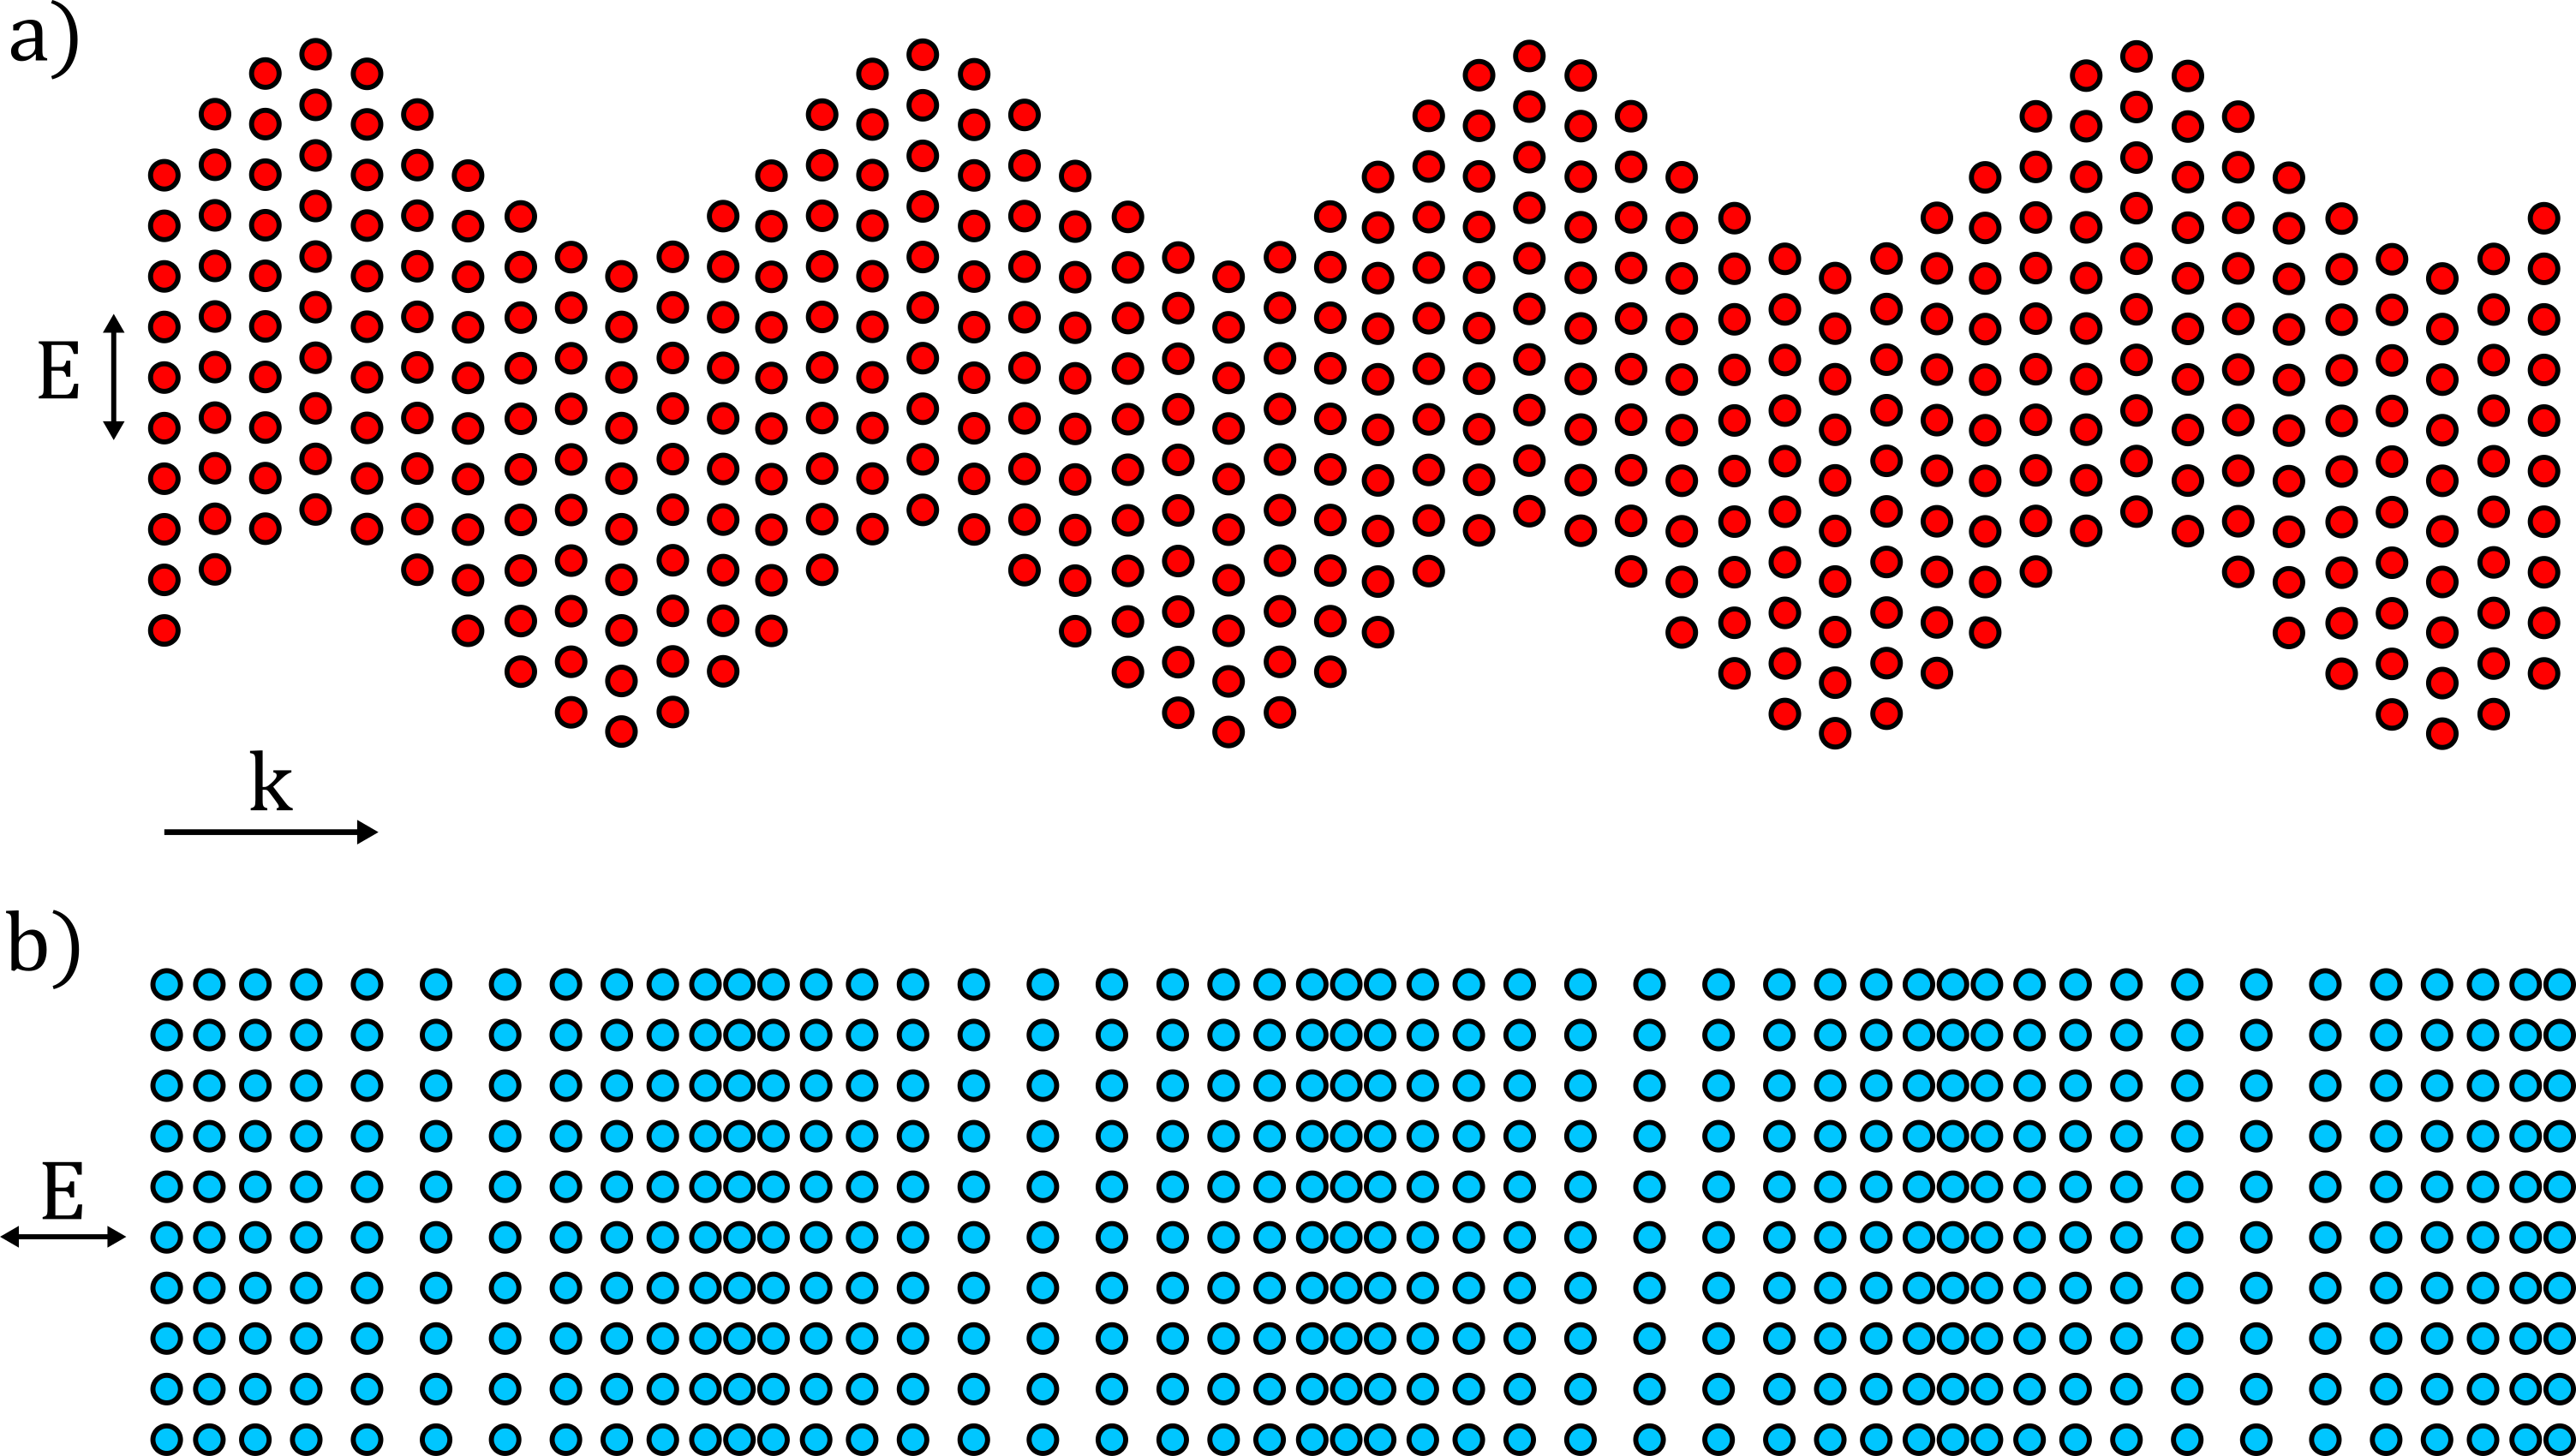
\includegraphics[width=0.75\linewidth]{Theory/Images/plasma_waves.png}
    \centering
    \caption{Particle motion in the electric fields of a) transverse and b) longitudinal plasma waves.}%
    \label{fig:theory_plasma_waves}
\end{figure}

In order to describe waves, the response of the plasma must be described in observable variables.
Here, the plasma is treated as a fluid, and is allowed to respond linearly to the applied fields.
An initially uniform, stationary plasma in equilibrium is considered with a number density for each species, $n_{\alpha 0}$.
The species is assumed to be isothermal or adiabatic, and therefore solution of the energy equation, Eq.~\ref{eq:theory_fluid_eqs_3} is not required.
An ideal gas equation of state is used to obtain a closure for the pressure in the momentum equation, Eq.~\ref{eq:theory_fluid_eqs_2},
\begin{equation}
    P_\alpha = n_\alpha T_\alpha = Cn_\alpha^{\gamma_\alpha},
\end{equation}
where $\gamma_\alpha$ is the adiabatic index of species $\alpha$ and $C$ is a constant.
In analogy to ideal gases, $\gamma_\alpha$ is related to the number of degrees of freedom of the fluid, for example, $\gamma_\alpha=1$ for an isothermal fluid and $\gamma_\alpha=3$ for an adiabatic fluid.
In this framework, the plasma response is completely described by a velocity ($\delta \vec{v}_\alpha$) and density ($\delta n_\alpha$) perturbation.
Linearising, we seek a solution to the following plasma response,
\begin{alignat}{2}
    n_\alpha(\vec{x},t) &= n_{\alpha 0} + \delta n_\alpha(\vec{x},t),&&\\
    \vec{v}_\alpha(\vec{x},t) &= \vec{v}_{\alpha 0} + \delta \vec{v}_\alpha(\vec{x},t) &&= 0 + \delta \vec{v}_\alpha(\vec{x},t),\\
    \vec{E}(\vec{x},t) &= \vec{E}_{0} + \delta \vec{E}(\vec{x},t) &&= 0 + \delta \vec{E}(\vec{x},t),\\
    \vec{B}(\vec{x},t) &= \vec{B}_{0} + \delta \vec{B}(\vec{x},t) &&= 0 + \delta \vec{B}(\vec{x},t),
\end{alignat}
where the subscript 0 quantities are the (constant) equilibrium values and $\delta\vec{E}=\vec{E}$ and $\delta\vec{B}=\vec{B}$ are the applied fields.
Inserting the linearised equations for each species into Eq.~\ref{eq:theory_fluid_eqs_1} (continuity equation) and Eq.~\ref{eq:theory_fluid_eqs_2} (momentum equation) it can be shown that in the absence of a magnetic field,
\begin{align}
    \label{eq:theory_wave1s_1}
    \frac{\delta n_\alpha}{n_{\alpha 0}} &= \frac{\vec{k}.\delta\vec{v}_\alpha}{\omega},\\
    \label{eq:theory_wave1s_2}
    \omega \delta\vec{v}_\alpha &= \gamma_\alpha v_{T\alpha}^2 \frac{\delta n_\alpha}{n_{\alpha 0}} \vec{k} + i\frac{q_\alpha}{m_\alpha}\vec{E},
\end{align}
where $\omega$ is the conjugate variable of time, $t$, from a Laplace transform and $\vec{k}$ is the conjugate variable of space, $\vec{x}$, from a Fourier transform.
The same equations can be obtained with a less formal treatment, by assuming a plane wave Ansatz for the perturbed quantities, $\delta\sim\exp{[i(\vec{k}.\vec{x} + \omega t)]}$.
These equations can then be combined to relate $\delta n_\alpha$ and $\delta \vec{v}_\alpha$ to $\vec{E}$,
\begin{align}
    \label{eq:theory_wave2s_1}
    \left[ \omega^2 - \gamma_\alpha v_{T\alpha}^2 k^2 \right]\frac{\delta n_\alpha}{n_{\alpha 0}} &= i \frac{q_\alpha}{m_\alpha} \vec{k}.\vec{E},\\
    \label{eq:theory_wave2s_2}
    \left[ \omega^2 - \gamma_\alpha v_{T\alpha}^2 \vec{k}(\vec{k}.) \right]\delta \vec{v}_\alpha &= i \frac{q_\alpha \omega}{m_\alpha} \vec{k}.\vec{E}.
\end{align}
Assuming a plane wave of the form $\vec{E}\propto \exp{\left[ i\left( \vec{k}.\vec{x} - \omega t \right) \right]}$, we identify $\vec{k}$ as the wavenumber and $\omega$ as the angular frequency.
Using the Ansatz that waves can either be transverse ($\vec{k}.\vec{E}=0$) or longitudinal ($\vec{k}\times\vec{E}=0$), dispersion relations in the fluid regime can be obtained for admissible solutions using these equations.
Fig.~\ref{fig:theory_plasma_waves}.a and Fig.~\ref{fig:theory_plasma_waves}.b plot the motion of particles under the influence of the electric field from each of these wave varieties.

%################################################################################
%################################################################################
\subsection{Electromagnetic Waves}%
\label{sec:theory_transwaves}

Firstly, the transverse wave solution shall be obtained, which is an \ac{EMW} propagating in the plasma.
Inserting the transverse wave Ansatz ($\vec{k}.\vec{E}=0$) into Eq.~\ref{eq:theory_wave2s_2} demonstrates that $\vec{k}.\delta\vec{v}_\alpha=0$, and therefore $\delta\vec{v}_\alpha = \delta\vec{v}_{\alpha\perp}$.
The transformed equation for the conservation of momentum, Eq.~\ref{eq:theory_wave1s_2} yields,
\begin{equation}
    \label{eq:theory_EMW_quiver}
    \delta\vec{v}_{\alpha\perp} = i \frac{q_\alpha}{m_\alpha \omega}\vec{E},
\end{equation}
which demonstrates that under the Lorentz force of the field, the particles undergo oscillatory `quiver' motion.
The quiver velocity of the ions is ignored because $m_i \gg m_e$ and therefore the ions are considered as a static background compared to the electron oscillations.
Therefore, the linearised current is only from the electron motion, $\sum\nolimits_\alpha\delta\vec{J}_\alpha\sim\delta\vec{J}_e = -e n_{e0}\delta \vec{v}_e = \sigma \vec{E}$.
Utilising the definition of the permittivity from Eq.~\ref{eq:theory_perm_def}, the plasma response to an \ac{EMW} is obtained,
\begin{alignat}{2}
    \label{eq:theory_emw_epsilon}
    \varepsilon &= 1 - \frac{\omega_p^2}{\omega^2} &&= 1- \frac{n_{e0}}{n_{\text{cr}}},\\
    \chi &= - \frac{\omega_p^2}{\omega^2}, &&
\end{alignat}
where the plasma frequency, defined previously in Eq.~\ref{eq:theory_plasma_freq}, has emerged.

\begin{figure}[t!]
    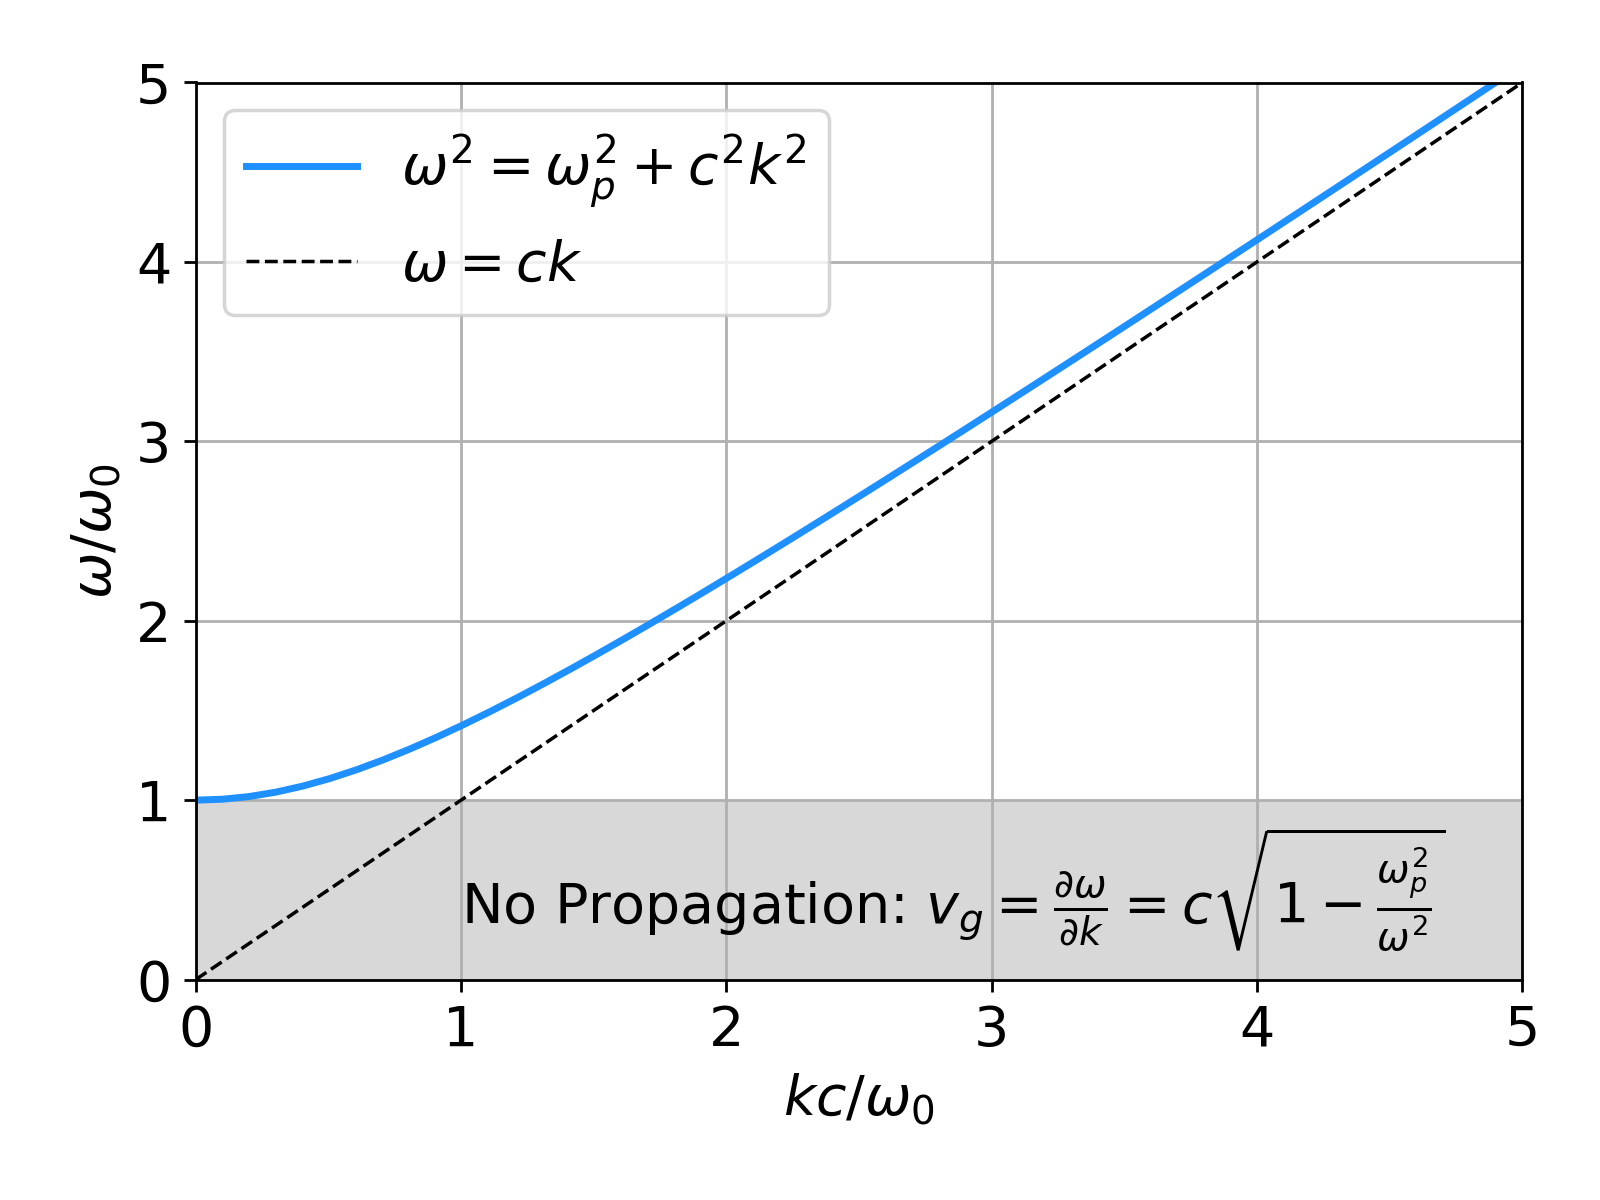
\includegraphics[width=0.6\linewidth]{Theory/Images/EMW_disp_rel.png}
    \centering
    \caption{The dispersion relation for an \ac{EMW} propagating in a plasma.
    For $\omega<\omega_p$, the oscillatory plane wave Ansatz turns into a decaying evanescent wave, thus the wave does propagate.}%
    \label{fig:EMW_disp_rel}
\end{figure}

A dispersion relation can also be obtained by utilising Maxwell's equations.
Taking the curl of Faraday's law (Eq.~\ref{eq:theory_maxwell_eqs_3}) and combining this with Amp\`ere's law (Eq.~\ref{eq:theory_maxwell_eqs_4}) to eliminate $\vec{B}$ yields,
\begin{equation}
    \label{eq:theory_manipulatedmaxwell}
    \left[ \partial_t^2 - c^2\nabla^2 + c^2 \nabla(\nabla.) \right]\vec{E} = -\frac{1}{\varepsilon_0}\partial_t \vec{J}.
\end{equation}
Assuming a plane wave Ansatz for $\vec{E}$ and inserting Eq.~\ref{eq:theory_emw_epsilon} to eliminate $\vec{J}$, the dispersion relation and wave equation for an \ac{EMW} are obtained,
\begin{align}
    \label{eq:emw_disp_rel}
    \omega^2 - \omega_p^2 - c^2 k^2 &= 0,\\
    \label{eq:theory_emw_wave_eq}
    \left( \partial_t^2 + \omega_{pe}^2 - c^2\nabla^2 \right)\vec{E}(\vec{x},t) &= 0.
\end{align}
The dispersion relation, Eq.~\ref{eq:emw_disp_rel}, is plotted in Fig.~\ref{fig:EMW_disp_rel}.
For $\omega<\omega_p$, $k$ becomes imaginary and therefore the plane wave Ansatz turns into a non-propagating, exponentially decaying evanescent wave.
The phase $v_\phi$ and group $v_g$ velocities of the light are also obtained from the dispersion relation,
\begin{alignat}{2}
    v_\phi &= \frac{\omega}{k} &&= \frac{c}{\sqrt{\varepsilon}},\\
    v_g &= \frac{\partial \omega}{\partial k} &&= \sqrt{\varepsilon} c,
\end{alignat}
which defines the refractive index of plasma, $n_{\text{ref}}=\sqrt{\varepsilon} = \sqrt{1-n_e/n_{\text{cr}}}$.
Note that $\sqrt{\varepsilon}<1$ so $v_\phi>c$.
However, the group velocity, which is the speed that information travels, remains subluminal.

%################################################################################
%################################################################################
\subsection{Plasma Waves}%
\label{sec:theory_longwaves}

\begin{figure}[t!]
    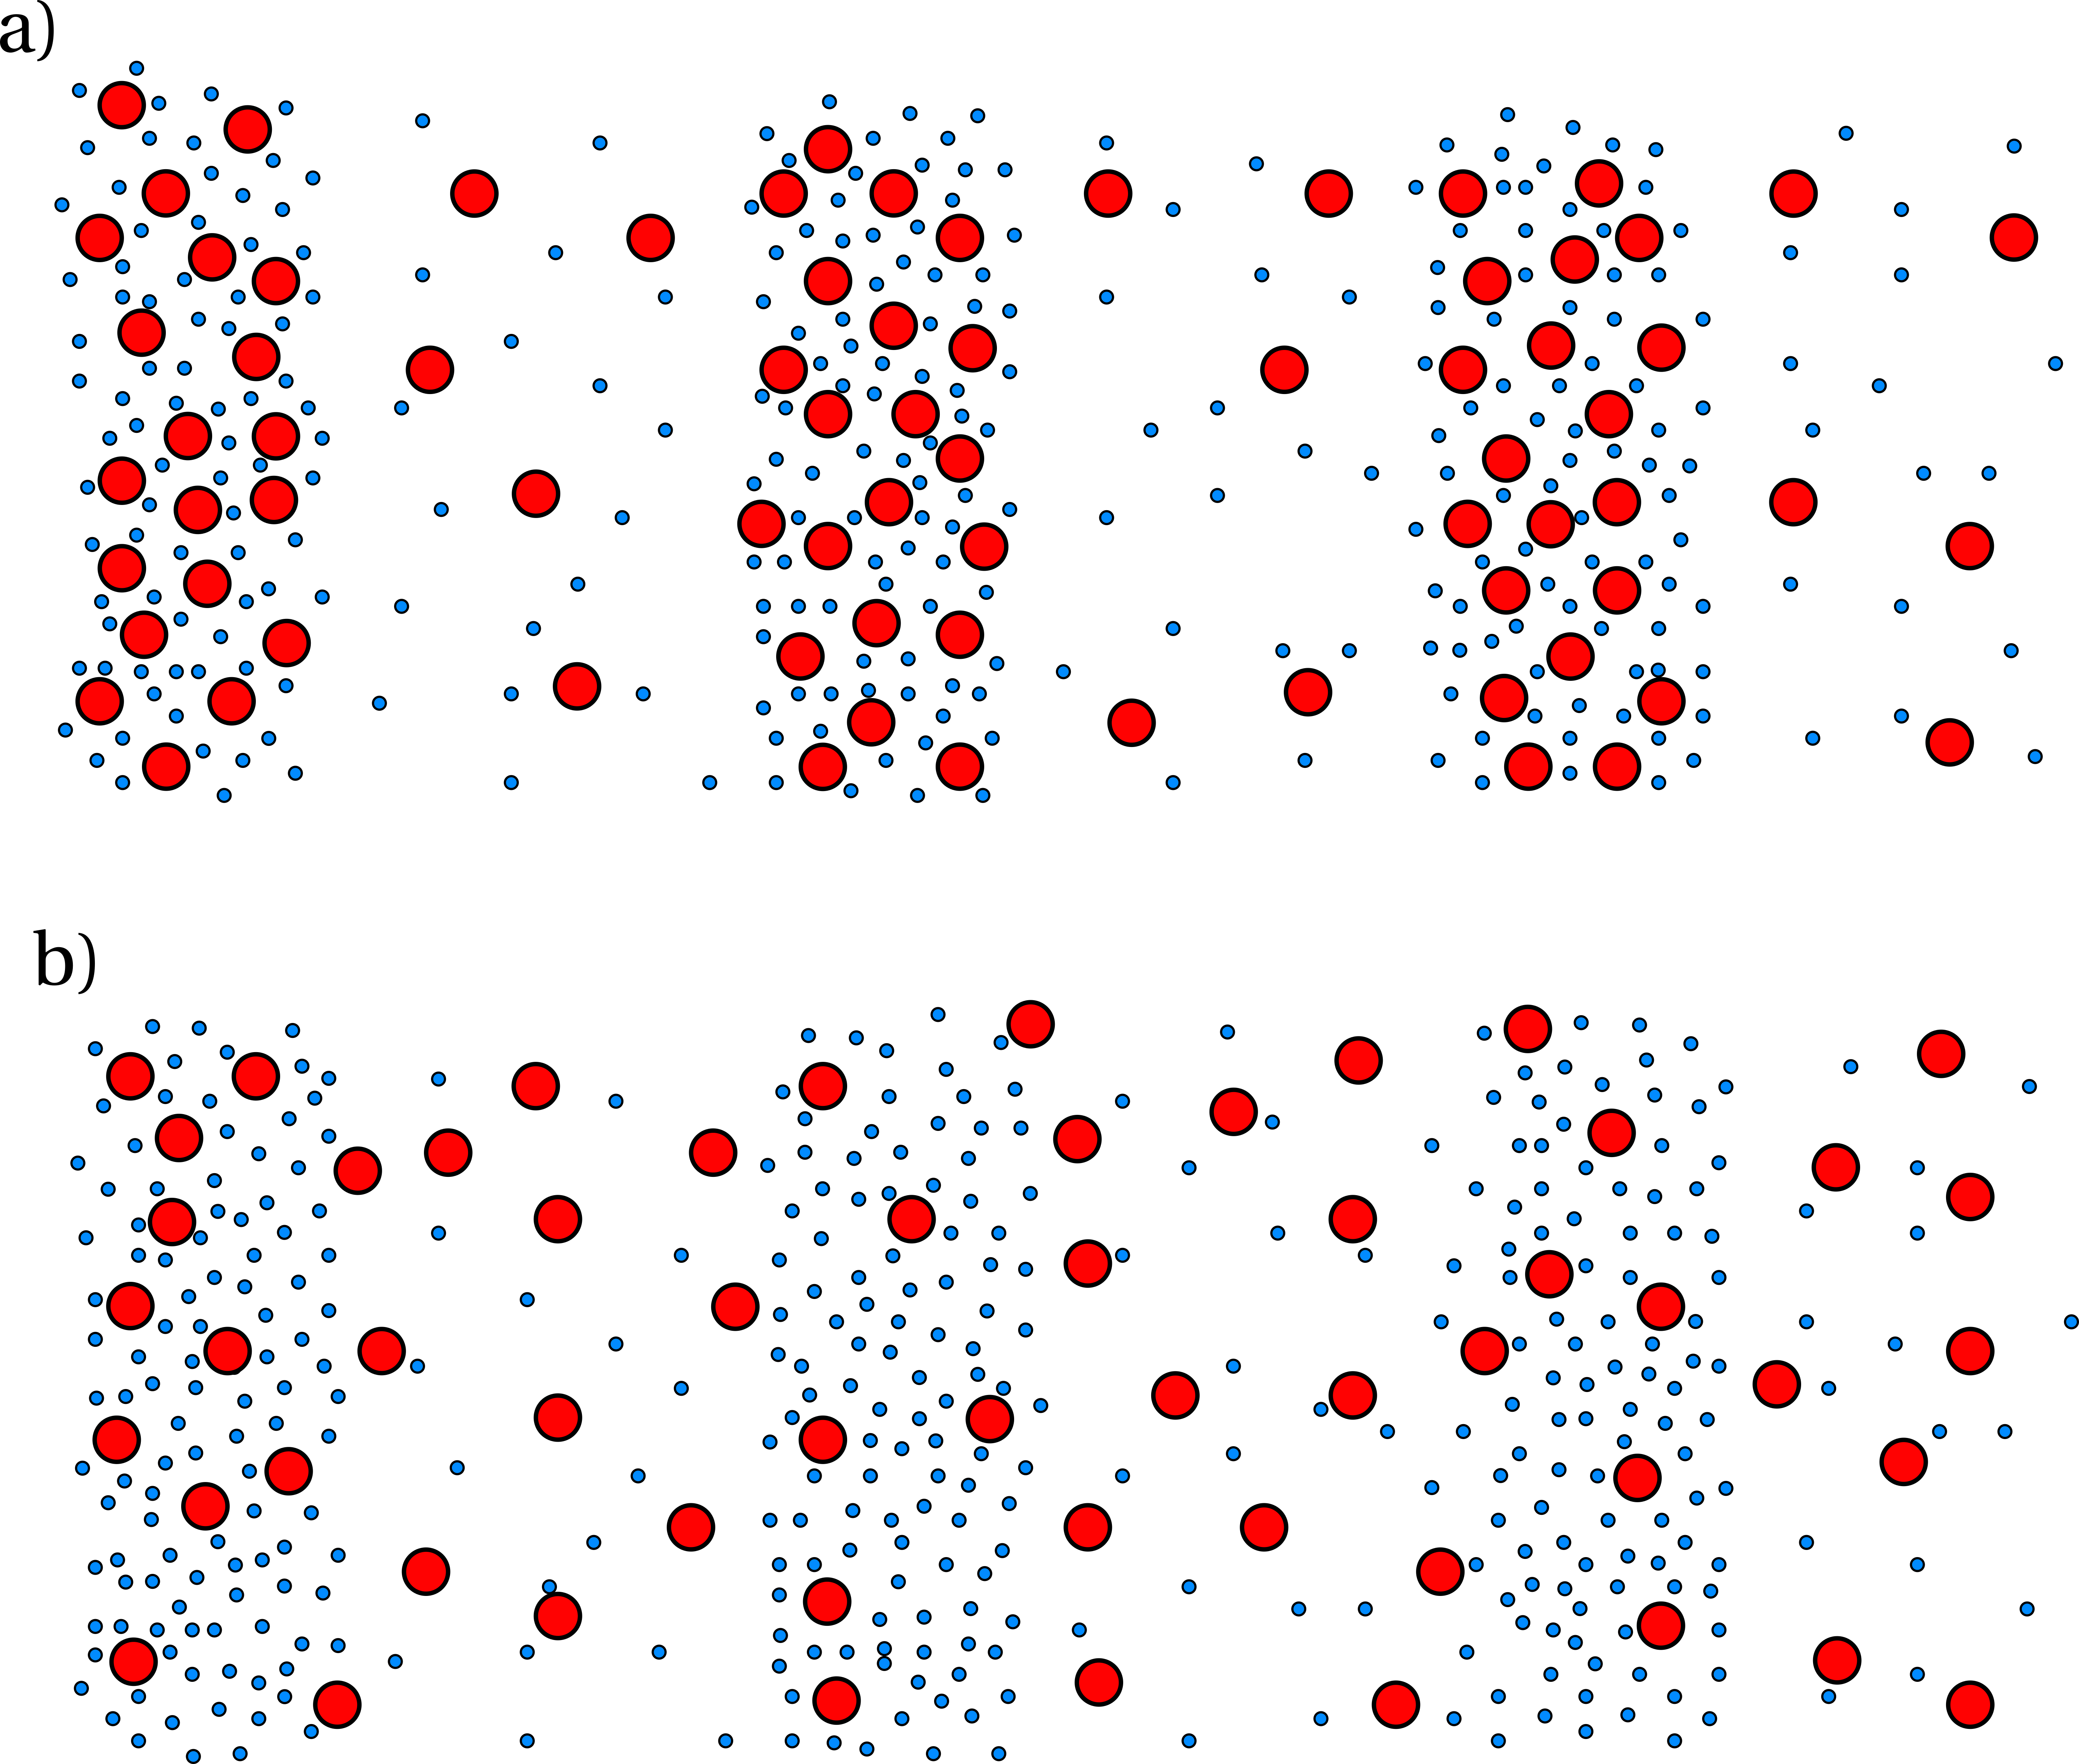
\includegraphics[width=0.7\linewidth]{Theory/Images/IAW_EPW.png}
    \centering
    \caption{Illustration of electron (small blue circle) and ion (large red circle) motion in a) an \ac{IAW} and b) an \ac{EPW}.}%
    \label{fig:theory_IAW_EPW}
\end{figure}

Two propagating longitudinal wave can exist in an unmagnetised plasma, an \ac{EPW}, which is an oscillation of the electron fluid on a timescale which is too fast for the ions to respond and an \ac{IAW}, which is a slower, joint oscillation of the electron and ion fluid.
The inertia of the \ac{EPW} and \ac{IAW} are set by the electron and ion masses respectively.
Electron pressure drives the \ac{EPW}, whereas both fluids contribute to the \ac{IAW} pressure, depending on the ionisation level of the plasma.
Fig.~\ref{fig:theory_IAW_EPW} illustrates particle motion in each wave.
Dispersion relations can be obtained similarly to the \ac{EMW} method from Sec.~\ref{sec:theory_transwaves}.
By first inserting the longitudinal Ansatz ($\vec{k}\times\vec{E}=0$) into Eq.~\ref{eq:theory_wave2s_2} to obtain the particle motion in a longitudinal wave,
\begin{equation}
    \delta \vec{v}_\alpha = i \frac{q_\alpha \omega}{m_\alpha} \frac{\vec{E}}{\omega^2 - \gamma_\alpha v_{T\alpha}^2 k^2}.
\end{equation}
Unlike the \ac{EMW}, we make no assumptions yet about which species contribute to the current, and thus the general form of the conductivity for longitudinal waves includes contributions from all species,
\begin{equation}
    \sigma = i\omega\varepsilon_0 \sum_{\alpha} \frac{\omega_{p\alpha}^2}{\omega^2 - \gamma_\alpha v_{T\alpha}^2 k^2},
\end{equation}
which yields the longitudinal wave permittivity and equivalently susceptibility,
\begin{align}
    \label{eq:long_permittivity}
    \varepsilon &= 1 + \sum_\alpha \chi_\alpha,\\
    \label{eq:long_susceptibility}
    \chi_\alpha  &= - \frac{\omega_{p\alpha}^2}{\omega^2 - \gamma_\alpha v_{T\alpha}^2 k^2}.
\end{align}
Inserting the plane wave Ansatz into~\ref{eq:theory_manipulatedmaxwell} (combined Faraday-Maxwell laws) and using Eq.~\ref{eq:long_permittivity} to eliminate $\vec{J}$ yields the generalised dispersion relation for longitudinal waves in a plasma,
\begin{equation}
    \label{eq:long_disp_rel}
    \varepsilon \vec{E} = 0.
\end{equation}
Further use of an Ansatz can be utilised to obtain a specific description of a particular plasma wave.
Note that unlike transverse waves, where $\delta n_\alpha=0$, which is seen by inserting $\vec{k}.\vec{E}=0$ into Eq.~\ref{eq:theory_wave2s_1} (particle density under the electric field of a wave), longitudinal waves do give rise to a density perturbation.
This can be heuristically understood by looking at Fig.~\ref{fig:theory_plasma_waves}, which illustrates particle bunching in an oscillatory, longitudinal electric field.
The charge separation from these longitudinal oscillations leads to an additional electric field component within the plasma, which is important for wave damping.

The longitudinal susceptibility (Eq.~\ref{eq:long_susceptibility}) has a pole at $\omega^2 = \gamma_\alpha v_{T\alpha}^2 k^2$, suggesting unbounded growth of the wave when its phase velocity is close to the thermal velocity of the species, $\alpha$.
This does not occur in actuality however, due to a process known as Landau damping, which is a resonant exchange of energy from the wave to particles.
When the phase velocity of the wave approaches this resonance, particles with velocity just below the group velocity, $|\vec{v}|\lesssim|\vec{v}_\phi|$, are trapped in the potential created by the charge separation and accelerated.
This transfers energy from the wave to the particles and thus prevents unbounded growth of the density perturbation.
Particles with velocity $|\vec{v}|\gtrsim|\vec{v}_\phi|$ are equivalently trapped and decelerated, leading to energy gain of the wave.
However, phase velocities of the plasma waves are greater than the thermal velocity where the fluid, Maxwellian distribution function peaks, and thus more particles are accelerated by this effect.
This energy gain of particles in longitudinal plasma waves is the basis for laser-plasma accelerators~\cite{tajima_laser_1979,esarey_physics_2009}.

%##########################################################
\subsubsection{Electron Plasma Waves}%
\label{sec:theory_EPWs}

Firstly the \ac{EPW} shall be considered.
These are fast oscillations of the electron fluid such that the heavier ions do not respond on the oscillation timescale.
To arrive at the dispersion relation, the assumption that the phase velocity is much faster than the electron thermal velocity is made, such that the wave can freely propagate without experiencing strong Landau damping, $w/k \gg v_{Te}$.
This assumption also yields $\lambda \gg v_{Te}/\omega$, which states that electrons travelling at the thermal velocity will not move a significant portion of the wavelength, $\lambda$, in one oscillation.
Temperature equilibration is thus limited throughout the wave, which means that there is no heat flux and such the electron fluid is assumed to be adiabatic.
An adiabatic fluid has $\gamma_e=3$, which is equivalent to a single degree of freedom in the motion.
Finally, the assumption is made that the ions are slow due to their large mass, and thus do not contribute to the permittivity.\footnote{Explicitly for the \ac{EPW}, $\omega/k \gg v_{Te} \gg v_{Ti}$ and thus $|\chi_e| \gg |\chi_i|$}
By using these assumptions in the generalised dispersion relation for longitudinal plasma waves, Eq.~\ref{eq:long_disp_rel}, the dispersion relation for the \ac{EPW} is obtained,
\begin{equation}
    \omega^2 = \omega_{pe}^2 + 3k^2v_{Te}^2.
\end{equation}
Just as for light waves, \ac{EPW} cannot propagate at $\omega\geq\omega_{pe}$.
The phase and group velocity of the wave are obtained from this dispersion relation,
\begin{alignat}{2}
    v_\phi &= \frac{\omega}{k} &&= v_{Te}\frac{\sqrt{1+3k^2\lambda_{D}^2}}{k\lambda_D},\\
    v_g &= \frac{\partial \omega}{\partial k} &&= 3v_{Te}\frac{k\lambda_D}{\sqrt{1+3k^2\lambda_{D}^2}}.
\end{alignat}

%##########################################################
\subsubsection{Ion Acoustic Waves}%
\label{sec:theory_IAWs}

The \ac{IAW} is of particular importance to the work conducted in this thesis, because it is the wave that mediates the energy exchange between light waves in \ac{CBET}.
To obtain the dispersion relation for this wave, the phase velocity of the wave is assumed to be much greater than the thermal velocity of the ions, but much less than the electron thermal velocity.\footnote{For the \ac{IAW}, $v_{Ti}\ll \omega/k \ll v_{Te}$.}
Using the same logic as the electrons in the \ac{EPW}, the ion fluid is assumed to be adiabatic, so $\gamma_i=3$.
The electrons, however, move much faster and can thus propagate over many wavelengths.
Therefore, they are able to equilibrate their temperature across the wave in a single oscillation, and are taken to be isothermal ($\gamma_e=1$).
When inserted into Eq.~\ref{eq:long_disp_rel}, these assumptions yield the dispersion relation,
\begin{equation}
    \omega^2 = \frac{k^2}{1 + k^2\lambda_D^2}\frac{ZT_e}{m_i} + 3 k^2 v_{Ti}^2.
\end{equation}
For oscillation wavelengths much larger than the Debye length, $k \lambda_D \ll 1$, this simplifies to,
\begin{equation}
    \omega \approx c_s k,
\end{equation}
where the sound speed is defined,
\begin{equation}
    c_s = \sqrt{\frac{Z k_B T_e + 3 k_B T_i}{m_i}}.
\end{equation}
The phase and group velocity of the light are simply $c_s$ in this limit, so the wave is non-dispersive.

Commonly in \ac{ICF}, plasmas are composed of multiple ion species, for instance the ablator of \textsc{Omega} targets is commonly composed of a CH plastic or SiO$_2$ glass shell.
The \ac{IAW} properties are typically greatly altered due to the additional susceptibility contributions from each species.
This leads to multiple \ac{IAW} modes with distinct speeds and damping.
Denoting the `heavy' and `light' ion species as $h$ and $l$ respectively, a fast ion mode exists when the phase velocity is greater than both ion thermal velocities,
\begin{equation}
    v_{Th} \leq v_{Tl} \ll v_{\phi,\text{fast}} \ll v_{Te}.
\end{equation}
A fast mode is also observed when only the heavy ion species is slower than the phase velocity,
\begin{equation}
    v_{Th} \ll v_{\phi,\text{slow}} \ll v_{Tl}  \ll v_{Te}.
\end{equation}
This is of particular relevance to the work in this manuscript, since \ac{CBET} in direct-drive typically occurs in multi-ion ablators, and it is moderated by an energy exchange via an \ac{IAW}.
Therefore, for example, different wave phenomena can affect the growth and saturation of energy transfer and must be accurately accounted for in computational modelling.
This is accounted for by the fluid and kinetic \ac{CBET} treatments, described in Sec.~\ref{sec:SOLAS_ray_power_change}.

%###############################################################################################################################
%###############################################################################################################################
%###############################################################################################################################
\section{Propagation and Absorption of Light in a Plasma}%
\label{sec:theory_propagation}

This section shall describe the propagation and absorption of light in plasma, in the regime of typical \ac{ICF} conditions.
Typically, sub-critical laser-driven \ac{ICF} plasmas can be treated as a linear medium and intensity of the light is sufficiently modest that it does not directly alter the refractive index of the plasma.
By making the WKB approximation, which is that over a wavelength the plasma may be treated as uniform, the equations of ray-tracing are derived.
Ray-tracing is the tool used to model lasers in the \textsc{Solas} module, the development of which is described in Chap.~\ref{chap:SOLAS}.
Absorption processes, which are important to energy deposition in laser-drive \ac{ICF} are then introduced, particularly collisional absorption, otherwise known as \ac{Inv-Brem}.
An absorption per-unit-length for \ac{Inv-Brem} is provided, which is suitable for integration along ray trajectories.

%################################################################################
%################################################################################
\subsection{The WKB Approximation}%
\label{sec:theory_WKB}

Laser-driven plasmas are heated and expand, leading to density gradients in the region where the light propagates.
The propagation path of the light through this plasma is governed by the refractive index, or equivalently permittivity, $\varepsilon = n_{\text{ref}}^2=1-n_e/n_{\text{cr}}$.
Thus, light refracts in plasmas with a density gradient.
Here, a description of light propagation through a non-uniform plasma (\textit{i.e.} $n_e = n_e(\vec{x})$) is obtained, in the limit that the plasma density does not vary significantly over the wavelength of the oscillation.
It is convenient to work with vector potentials, $\vec{B} = \nabla\times\vec{A}$ and $\vec{E} = -\partial_t\vec{A}$, rather than electric field for laser-plasma waves.\footnote{Note that the Coulomb gauge has been used here, $\nabla.\vec{A}=0$, otherwise $\vec{E}=-\partial_t\vec{A}-\nabla\phi$, where $\phi$ is the scalar potential.}
This is because electric fields can describe both longitudinal and transverse waves, whereas the vector potential is purely for transverse oscillations and as such cannot describe plasma waves.
Using the vector potential, the \ac{EMW} wave equation, Eq.~\ref{eq:theory_emw_wave_eq}, can be rederived from Maxwell's equations,
\begin{equation}
    \label{eq:theory_waveeq_a}
    \left( \partial_t^2 + \omega_{pe}^2 - c^2\nabla^2 \right)\vec{a} = 0,
\end{equation}
where the normalised vector potential is defined,
\begin{equation}
    \vec{a} = \frac{e}{\omega m_e c}\vec{A},
\end{equation}
where $\omega$ is the angular frequency of the light wave.
The light is said to be relativistic when $|\vec{a}|\sim1$, because $|\vec{a}|$ is equivalent to the maximum quiver velocity of an electron divided by the speed of light.
If the wave propagates normally up a plasma density gradient (aligned with $z$), polarisation of the wave can be ignored by rotational symmetry and a solution can be sought of the form,
\begin{equation}
    \label{eq:theory_fz}
    a(z,t) = \frac{1}{2} f(z) a_0e^{-i\omega t} + c.c.,
\end{equation}
where $a_0$ is the oscillation amplitude, $c.c.$ is the complex conjugate and $f(z)$ is the spatial dependence of the oscillation.
In this limit, the WKB (for Wentzel, Kramers, Brillouin) approximation can be used to find a solution for $f(z)$.

Inserting Eq.~\ref{eq:theory_fz} into the wave equation, Eq.~\ref{eq:theory_waveeq_a}, yields the 1-D Helmholtz equation,
\begin{equation}
    \label{eq:theory_Helmholtz}
    \left[ \partial_z^2 + \varepsilon(z)k_0^2 \right] f(z) = 0,
\end{equation}
where $k_0=\omega/c$ is the vacuum wavenumber.
The Helmholtz equation describes the steady state propagation of light through a plasma, which is defined by the permittivity, $\varepsilon$.
An Ansatz is used~\cite{michel_introduction_2023},
\begin{equation}
    \label{eq:theory_Helmholtz_ansatz}
    f(z) = e^{i k_0 \varphi (z)},
\end{equation}
where $\varphi$ is a series expansion~\cite{colaitis_modeling_2014},
\begin{equation}
    \label{eq:theory_S_expansion}
    \varphi(z) = \left[ S_0 (z) + \frac{S_1 (z)}{i k_0} + \frac{S_2 (z)}{(i k_0)^2} + \dots \right],
\end{equation}
which is valid so long as the expansion parameter is large, $k_0 \gg |\nabla \varepsilon|/\varepsilon$, which is shown explicitly at the end of the section.

By combining Eqs.~\ref{eq:theory_Helmholtz},~\ref{eq:theory_Helmholtz_ansatz} and~\ref{eq:theory_S_expansion} and keeping only the dominant, $\mathcal{O}\left(k_0^{n=0}\right)$ terms, the expression for the first order expansion term is obtained,
\begin{equation}
    S_0(z) = \pm \int_0^z \sqrt{\varepsilon(z)}\ \text{d}z.
\end{equation}
If only this term is kept and there is a uniform plasma (therefore $\varepsilon$ is constant), then a plane wave propagating solution is obtained for the field,
\begin{equation}
    a(z,t) = \frac{a_0}{2} \exp{\left[  i (\pm k_0 z - \omega t )\right]}.
\end{equation}
If the next order terms, $\mathcal{O}\left(k_0^{n=-1}\right)$, are collected and equated, then the following expression is retrieved,
\begin{equation}
    S_1(z) = i \ln{\left( \varepsilon^{1/4} \right)} + \varphi_0,
\end{equation}
where $\varphi_0$ is an integration constant, identified as the initial phase of the light.
Note that in this work, the \textit{dimensional} phase is used, such that the phase terms $\varphi$, have spatial units.
This is often convenient to work with, because the parametric variables of phase, path and arc length all share the same dimension.
The \textit{dimensionless} phase is obtained by multiplication with the vacuum wavenumber, $\psi \equiv k_0 \varphi$.
An expression for the light field is obtained by keeping the next order terms~\cite{michel_introduction_2023},
\begin{equation}
    \label{eq:theory_WKB_rayfield}
    a(z,t) = \frac{1}{2}\frac{a_0}{\varepsilon^{1/4}}\exp{ \left[ \pm i \int_0^z k(z) \text{d}z - i\omega t +ik_0\varphi_0 \right] } + c.c,
\end{equation}
where $k(z)=\sqrt{\varepsilon(z)}k_0$.
The $\varepsilon^{1/4}$ term outside the exponential leads to higher field in regions of the plasma with higher densities and is known as `field-swelling'.
It occurs due to the reduced group velocity of light at lower $\varepsilon$ values, resulting in a pile up of field as light propagates up a density gradient.
The validity condition of the WKB solution in Eq.~\ref{eq:theory_WKB_rayfield} can be demonstrated by mandating that the $\mathcal{O}\left(k_0^{n=-2}\right)$ terms from the expansion are much smaller than the $\mathcal{O}\left(k_0^{n=-1}\right)$ terms.
This leads to the validity domain (for the normally incident light considered here),
\begin{equation}
    \frac{|\nabla \varepsilon|}{\varepsilon} \ll k,
\end{equation}
where, stated again for emphasis, $k=\sqrt{\varepsilon}k_0$.
In other words, the length scale $L$ associated with $\nabla\varepsilon$ must be far larger than the oscillation wavelength $\lambda = 2\pi/(k_0\sqrt{\varepsilon})$.
This condition is violated either for plasmas with extreme density gradients, or in a narrow region near the critical surface, where the oscillation wavelength grows to infinity.
When calculating field amplitudes under the WKB approximation therefore, specialised treatments are required in the region close to the critical surface (or turning point of the light when it is not normally incident), as is shown explicitly in Sec.~\ref{sec:SOLAS_ray_amplitude}.

%################################################################################
%################################################################################
\subsection{Ray-Tracing}%
\label{sec:theory_rays}

The WKB approximation correctly captures the behaviour of light, apart from a narrow region near the wave turning point.
Ray-tracing is a technique, which provides a framework to integrate the WKB solution along the trajectory of the light, at discrete points on an initial phase front.
This turns out to be a highly useful tool for numerical implementation of laser modelling.
Starting from the Helmholtz equation, now generalised to multiple dimensions~\cite{colaitis_modeling_2014},
\begin{equation}
    \left[ \nabla^2 + \varepsilon(\vec{x})k_0^2 \right] a(\vec{x}) = 0,
\end{equation}
a solution is sought of the form,
\begin{equation}
    a(\vec{x}) = A(\vec{x}) e^{i k_0 \varphi(\vec{x})} \equiv A(\vec{x}) e^{i \psi(\vec{x})},
\end{equation}
where going from 1-D$\rightarrow$3-D, we have made the change $f(z)\rightarrow A(\vec{x})$, where $A(\vec{x})$ is now called the `ray-amplitude'.
Similarly to Sec.~\ref{sec:theory_WKB}, $\varphi(\vec{x})$ is expanded, and the Ansatz is inserted into the Helmholtz equation, which returns the following equations:
\begin{align}
    \label{eq:theory_eikonal_eq}
    \left[\nabla \varphi(\vec{x})\right]^2  - \varepsilon(\vec{x}) &= 0,\\
    \label{eq:theory_transport_eq}
    2\left[\nabla A(\vec{x}) . \nabla \varphi (\vec{x}) \right] + A(\vec{x}) \nabla^2 \varphi(\vec{x}) &= 0,
\end{align}
where Eq.~\ref{eq:theory_eikonal_eq} is known as the Eikonal equation, and Eq.~\ref{eq:theory_transport_eq} is known as the transport equation.
So far, this is simply a multidimensional corollary of the same procedure that was followed in Sec.~\ref{sec:theory_WKB}.

The ray-tracing equations are obtained by noticing that Eq.~\ref{eq:theory_eikonal_eq} describes the Hamiltonian of a system,
\begin{equation}
    \mathcal{H} = \frac{1}{2} \left[ \vec{p}^2 - \varepsilon(\vec{x}) \right],
\end{equation}
which has a momentum $\vec{p} = \nabla \varphi(\vec{x})$, and a potential $-\varepsilon(\vec{x})$.
Thus, using the characteristic technique, the following equations of motion are obtained,
\begin{align}
    \label{eq:theory_ray_x}
    \frac{\text{d} \vec{x}}{\text{d} \tau}&=\vec{p}, \\
    \label{eq:theory_ray_k}
    \frac{\text{d} \vec{p}}{\text{d} \tau}&=\frac{1}{2} \nabla \varepsilon(\vec{x}),
\end{align}
which describe the evolution of a wave packet (typically called a ray) along its optical path length, $\tau$, through a medium defined by $\varepsilon(\vec{x})$~\cite{colaitis_modeling_2014}.
The wavevector is simply related to this momentum $\vec{k}=k_0\vec{p}$.
Similarly to the WKB solution, it is valid as long as the evolution of the envelope function, \textit{i.e.} the ray amplitude $A(\vec{x})$, are slow compared to the spatial oscillations described by $|\vec{k}|$.
These equations can be readily integrated along $\tau$ to describe the trajectory of the field, from a discrete initial point on its initial surface.

The evolution of the ray amplitude is obtained by integrating the transport equation, Eq.~\ref{eq:theory_transport_eq},
\begin{align}
    \label{eq:theory_ray_amp}
    A(\tau) &= A(0)\left| \frac{D(0)}{D(\tau)} \right|^{1/2}, \\
    D(\tau) &= 
    \begin{bmatrix}
        \frac{\partial x}{\partial \zeta_1} & \frac{\partial x}{\partial \zeta_2} & \frac{\partial x}{\partial \tau} \\
        \frac{\partial y}{\partial \zeta_1} & \frac{\partial y}{\partial \zeta_2} & \frac{\partial y}{\partial \tau} \\
        \frac{\partial z}{\partial \zeta_1} & \frac{\partial z}{\partial \zeta_2} & \frac{\partial z}{\partial \tau}
    \end{bmatrix},
\end{align}
where $[x,y,z]$ and $[\zeta_1,\zeta_2,\tau]$ are the ray real-space and phase-space coordinates respectively and $D(\tau)$ is the Jacobian for the coordinate transform from phase-space to real-space~\cite{colaitis_inverse_2021}.
Physically, the phase space coordinate $\tau$ represents the distance along a wave packet trajectory, and $[\zeta_1,\zeta_2]$ are the initial position of the wave packets on the 2-D beam port ($\tau=0$).
This represents the conservation of energy along a tube of the light, defined by an infinitesimally small separation of rays.
Here, infinitesimally small means that it is small compared to the spatial variations of the medium, $L\sim|\varepsilon/\nabla \varepsilon|$.
Unlike Eqs.~\ref{eq:theory_ray_x} and~\ref{eq:theory_ray_k}, it is not immediately obvious how to integrate this equation along a ray path.
The solution method taken in this manuscript is to trace a small bundle of rays and calculate their separation at discrete points along the path, which is described in more detail in Sec.~\ref{sec:SOLAS_ray_amplitude}.

Temporal variation of the medium may also affect the evolution of the field.
For most \ac{HEDP} experiments, the time taken for light to traverse the region of interest is small compared to the temporal evolution of $\varepsilon$, therefore it is usually safe to disregard its effect.
One exception to this is \ac{LPIs}.
The mechanism for these instabilities is described in more detail in Sec.~\ref{sec:theory_LPIs}, but they can rely on a precisely matched \ac{EMW} frequency condition to excite.
Therefore, even small differences to wave frequencies can lead to errors in modelling.
The evolution of the frequency of the light is obtained from the dispersion relation~\cite{dewandre_doppler_1981},
\begin{equation}
    \frac{\text{d}\omega^2}{\text{d}t} = \frac{\text{d}\omega_p^2}{\text{d}t}.
\end{equation}
This leads to an equation for the integration along ray trajectories,
\begin{equation}
    \label{eq:theory_doppler}
    \frac{\text{d} \omega}{\text{d} \tau}=\frac{\omega}{2 c} \frac{\partial\left(n_e / n_{\text{cr}}\right)}{\partial t},
\end{equation}
where $\text{d}t = \text{d}\tau/c$.
Eq.~\ref{eq:theory_doppler} describes the temporal bunching or rarefaction of successive wavefronts propagating at a discrete point in space, due to a temporally increasing or decreasing refractive index.
The evolution timescale is typically long for \ac{ICF} compared $1/\omega$ and therefore the percentage change of $\omega$ is small.
Eq.~\ref{eq:theory_doppler} can thus be evolved independently of Eqs.~\ref{eq:theory_ray_x} and~\ref{eq:theory_ray_k}.
In direct-drive \ac{ICF} experiments, evolution of the coronal plasma can be diagnosed by measuring this frequency shift~\cite{seka_timeresolved_2008}.

%################################################################################
%################################################################################
\subsection{Inverse-Bremsstrahlung}%
\label{sec:theory_in_brem}

\begin{figure}[t!]
    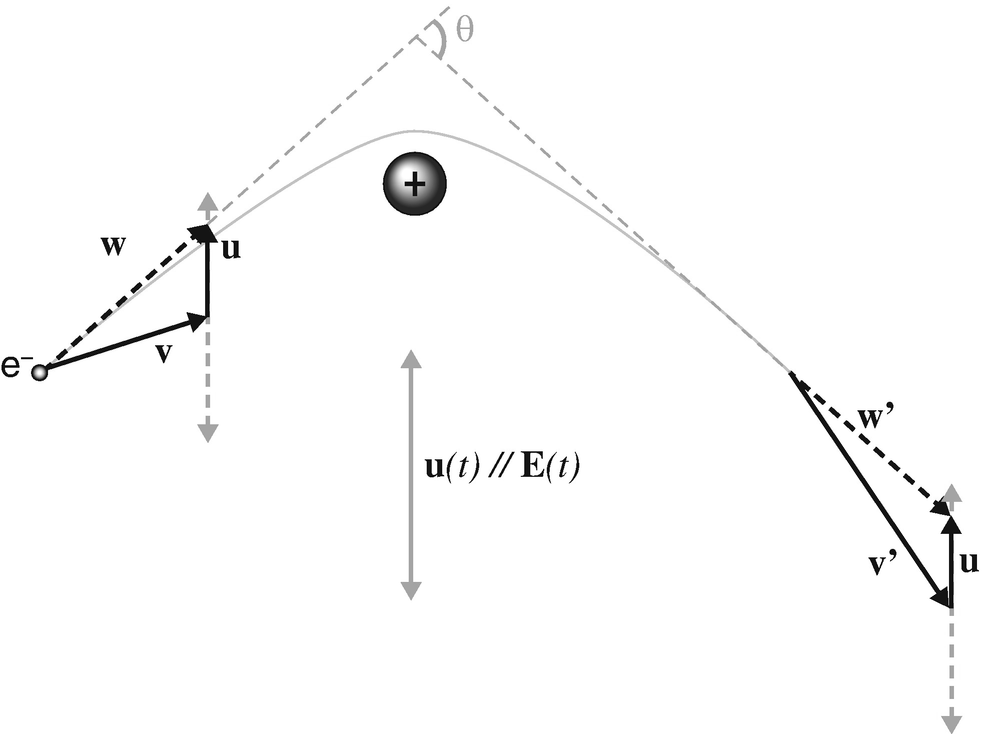
\includegraphics[width=0.6\linewidth]{Theory/Images/Inv_Brem.png}
    \centering
    \caption{An electron-ion collision in the presence of an oscillating electric field.
    The collision time is much shorter than the oscillation time.
    The magnitude of the electron velocity just before ($\vec{w}$) and just after ($\vec{w}'$) the collision is the same, since the collision is elastic.
    However, the electron continues its quiver motion ($\vec{u}$) just after the collision and thus the time-averaged velocities before ($\vec{v}$) and after ($\vec{v}'$) are different.
    The figure has been reproduced with permission from Ref.~\cite{michel_introduction_2023}.}%
    \label{fig:theory_inv_brem}
\end{figure}

Lasers are used in \ac{HEDP} experiments as an energy source, which drives the plasma dynamics.
The energy from the laser must therefore be absorbed into the plasma to drive this motion.
\ac{Inv-Brem}, otherwise known as collisional absorption, is the dominant heating mechanism for modern direct-drive experiments.
This is the absorption of wave energy by the electron population of the plasma as they undergo collisions with the ions.
Collisions with the ions are required for energy transfer from the wave to the electrons, as without collision, the electrons would simply gain and lose energy cyclically as they oscillated in the laser electric field.
When collisions with ions are included, electrons are deflected, disrupting their cyclical quiver energy exchange.
Therefore, the full portion of kinetic energy that an electron gains from a quiver oscillation, is not restored to the field, resulting in damping of the wave and net energy gain of the electron population.

The physical picture of the absorption process is outlined in Fig.~\ref{fig:theory_inv_brem}.
In this figure, an electron undergoes a collision with an ion, while oscillating in an electric field.
The total motion of the electron, $\vec{w}$, is described by a quiver component, $\vec{u}$, and a guiding centre component, $\vec{v}$, which is averaged over the oscillatory motion,
\begin{equation}
    \vec{w} = \vec{v} + \vec{u},
\end{equation}
where $|\vec{u}| = e|\vec{E}|/m_e \omega$ is the quiver velocity of the electrons in the field, defined in Eq.~\ref{eq:theory_EMW_quiver}.
The thermal energy of the population is effectively the randomly distributed velocities, $\vec{v}$, which is a Maxwellian if the plasma is in equilibrium.
The quiver velocity of the electrons is thus effectively a guiding centre drift of a Maxwellian compared to a stationary ion population, which relaxes to a Maxwellian by collisions with the ions.
An equation of motion for the quiver component can therefore be written,\footnote{Note that only the dominant terms in an expansion around the `small' parameter, $|\vec{u}|/|\vec{v}|\equiv v_\text{quiv.}/v_{Te}$ have been kept. It has been shown that the following \ac{Inv-Brem} absorption rate is valid for $v_\text{quiv.}/v_{Te}\leq 1$~\cite{bunkin_interaction_1973}.}
\begin{equation}
    \label{eq:theory_electron_quiver_partial}
    \frac{\partial\vec{u}}{\partial t} = - \frac{e}{m_e}\vec{E} - \nu_{ei} \vec{u},
\end{equation}
where $\nu_{ei}$ is the electron-ion collision rate~\cite{michel_introduction_2023},
\begin{equation}
    \nu_{ei} = \frac{2 n_i}{\sqrt{2\pi} m_e^2 v_{Te}^3} \left( \frac{Z e^2}{4 \pi \varepsilon_0} \right)^2 \frac{4\pi}{3} \ln{\left(\Lambda\right)}.
\end{equation}
The Coulomb logarithm, $\ln(\Lambda)$, is the logarithm of the ratio of minimum and maximum impact parameters for a collision.
Its expression takes different forms for different physical effects.
When considering a quivering electron, oscillating in an electric field, the appropriate form for $\Lambda$ is,
\begin{align}
    \Lambda &= \frac{v_{Te}}{V},\\
    V &= \text{max}\left( \omega, \omega_p \right) \times \text{max}\left( \frac{Z e^2}{k_B T_e}, \frac{\hbar}{\sqrt{m_e k_B T_e}} \right),
\end{align}
where $\hbar$ is the reduced Planck constant~\cite{huba_nrl_2013}.

Assuming a plane wave solution, ($\vec{E},\vec{v}\propto \exp{(i\omega t)}$), an expression for the quiver velocity is found from Eq.~\ref{eq:theory_electron_quiver_partial},
\begin{equation}
    \vec{u} = \frac{-ie}{m(\omega + i\nu_{ie})}\vec{E}.
\end{equation}
Recalling the definition of the current, $\vec{J}_e = -e n_e \vec{u} = -i\omega \varepsilon_0 \chi_e$, the permittivity ($\varepsilon = 1-\chi_e$) is found to be,
\begin{equation}
    \varepsilon = 1 - \frac{\omega_p^2}{\omega^2 + i \omega\nu_{ei}}.
\end{equation}
In the small absorption limit, where $\nu_{ei}\ll \omega$, the wavevector, $k = \sqrt{\varepsilon}\omega/c$ is complex,
\begin{equation}
    k = \frac{\omega}{c}\sqrt{\varepsilon} + i\frac{1}{2}\frac{\nu_{ei}}{c\sqrt{\varepsilon}}\frac{n_e}{n_{\text{cr}}}.
\end{equation}
The small absorption limit is generally valid for the hot coronal plasmas of direct-drive \ac{ICF} experiments, apart from in a thin region close to the critical surface~\cite{colaitis_real_2019}.
The imaginary component describes a damping of the wave amplitude as it propagates in space, with an absorption rate per $\text{d}\tau$,
\begin{equation}
    \label{eq:theory_inv_brem}
    \kappa_{\text{IB}} = 2 \frac{\nu_{ei}}{c}\frac{n_e}{n_{\text{cr}}},
\end{equation}
where the $\sqrt{\varepsilon}$ drops out when converting from unit arc length to path length.

One further improvement can be made to Eq.~\ref{eq:theory_inv_brem}, by noting that \ac{Inv-Brem} preferentially heats the colder population of electrons, because the collision frequency $\nu_{ei}\propto v^{-3}$.
If the heating rate is fast compared to the collisional rate which returns the distribution function to Maxwellian, then this can lead to super-Gaussian distribution functions.
These distributions have a lower population of the cold electrons, therefore the overall absorption rate is decreased.
This process is known as the Langdon effect~\cite{langdon_nonlinear_1980} and is parameterised by the ratio of the heating rate to the thermalising the electron-electron collision rate,
\begin{equation}
    \label{eq:theory_alpha_langdon}
    \alpha = Z^* \frac{v_{\text{quiv}}^2}{v_{Te}^2},
\end{equation}
where $Z^* = \langle Z^2 \rangle / \langle Z \rangle $ (the average is taken over multiple ion species if present) and $v_{\text{quiv.}} = e|\vec{E}|/m_e \omega$ is the quiver velocity.
The modified absorption kernel is then the value from Eq.~\ref{eq:theory_inv_brem}, multiplied by the factor~\cite{colaitis_inverse_2021},
\begin{equation}
    f_{\text{L}} = \left[ 1 - 0.553/\left( 1 + {[0.27/\alpha]}^{0.75} \right) \right].
\end{equation}
One issue with accurately implementing this effect in a ray-tracing code is that the field along each ray must be known to calculate $v_{\text{quiv.}}$, and therefore the amplitude of the ray must be integrated, which is not trivial.

%################################################################################
%################################################################################
\subsection{Resonance Absorption}%
\label{sec:theory_res_abs}

\begin{figure}[t!]
    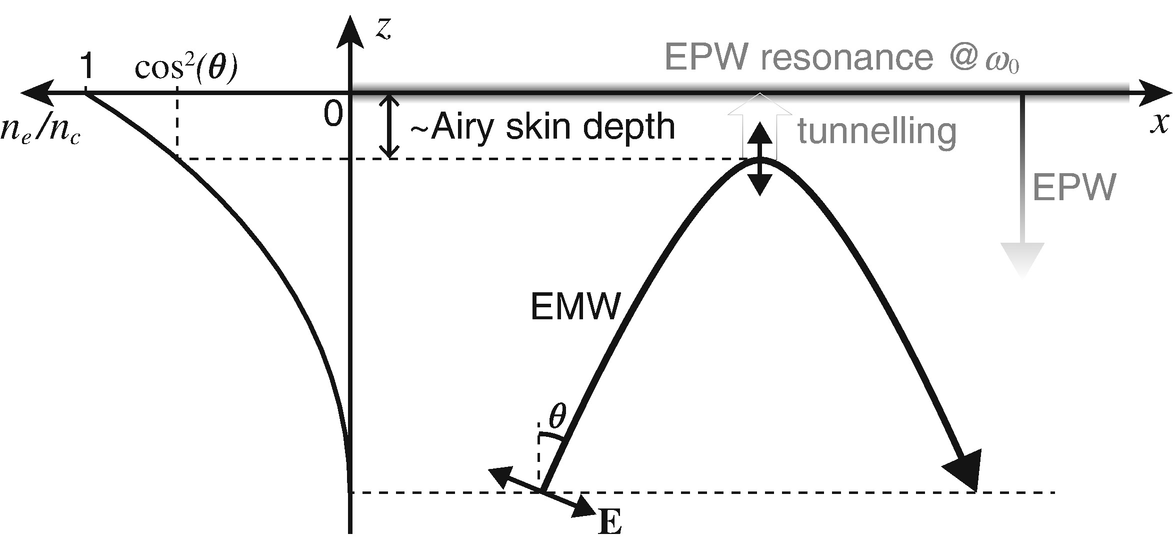
\includegraphics[width=0.65\linewidth]{Theory/Images/Res_Abs.png}
    \centering
    \caption{Illustration of resonance absorption for a non-normally incident, p-polarised light wave, propagating up a density gradient.
    At the turning point of the light, if sufficiently close to the critical density, then the evanescent light can tunnel through to the critical surface and resonantly excite an \ac{EPW}.
    The \ac{EPW} propagates down the density ramp and transfers energy to the electrons through damping.
    The figure has been reproduced with permission from Ref.~\cite{michel_introduction_2023}.}%
    \label{fig:theory_res_abs}
\end{figure}

An additional absorption mechanism is also important for many \ac{HEDP} experiments, known as resonance absorption.
This mechanism is far less important for direct-drive experiments on \textsc{Omega} and the \ac{NIF}, due to the use of frequency tripled light and long plasma scale lengths, however a short discussion is included for completeness.
An illustration of the procedure is shown in Fig.~\ref{fig:theory_res_abs}.
Light propagating up a density gradient, reaches a maximum plasma density of $n_e = n_{\text{cr}} \cos{\theta}$, where $\theta$ is the angle of the light to the density gradient.
If the light is p-polarised, then the field oscillates in the plane of the gradient, therefore a finite portion of the evanescent field is able to tunnel through to the critical density.
This field will resonantly excite an \ac{EPW} at the frequency of the light wave, which propagates down the density gradient.
As it propagates down, the \ac{EPW} will irreversibly lose energy to the plasma via Landau damping or collisional damping, resulting in laser energy absorption by the plasma.

If the light is normally incident to the density ramp, then the field is purely s-polarised, thus no resonance absorption can occur.
However, the light must propagate sufficiently close to normal incidence in order to get close to the critical surface.
This places strict requirements on plasma conditions and laser propagation for resonance absorption to be significant compared to \ac{Inv-Brem}.
In long density length scale plasmas, only a very small portion of the incident laser light gets sufficiently close to the critical surface for large portions of resonance absorption to occur.
Additionally, \ac{Inv-Brem} often dominates apart from when it becomes ineffective at high plasma temperatures.
It can however be a significant absorption mechanism for short length and timescale, high intensity laser-solid interactions, before the target has significantly heated and expanded.
Specifically for \ac{ICF} however, resonance absorption is thought to be mostly insignificant on \textsc{Omega} since the move to frequency tripled lasers~\cite{craxton_directdrive_2015}.

%###############################################################################################################################
%###############################################################################################################################
%###############################################################################################################################
\section{Laser Plasma instabilities}%
\label{sec:theory_LPIs}

This section shall provide some introductory theory which is required to understand \ac{LPIs}.
The ponderomotive force is introduced, which is the mechanism by which crossing light waves are able to excite longitudinal plasma waves and thus lead to \ac{LPIs}.
A quantitative picture of these three-wave coupling processes is provided, which describes how the plasma waves are produced and act to scatter the light waves.
The specific mechanism for \ac{CBET} is described and the gain, which is the rate at which each \ac{EMW} gains or loses energy, is provided in the limit of a fluid description of the plasma.
The effect of \ac{CBET} in \ac{ICF} experiments is discussed and some further modifications to the simple picture provided are given, such as the Langdon effect of \ac{Inv-Brem} heating on the \ac{CBET} gain.

%################################################################################
%################################################################################
\subsection{The Ponderomotive Force}%
\label{sec:theory_ponderomotive }

When interacting with a wave that has a non-uniform envelope, plasma particles undergo a drift from the regions of high field amplitude to low amplitude, on top of their fast quiver motion.
This effect is known as the ponderomotive force and is crucial to the development of \ac{LPIs}.
Although the ponderomotive force acts on particles in both longitudinal and transverse waves in plasmas, this section shall focus only on the effect due to an \ac{EMW}.
Considering an \ac{EMW} with a non-uniform envelope, polarised along the $\pm \hat{\vec{x}}$ axis and propagating along $+\hat{\vec{z}}$, the electric field of the wave can be written,
\begin{equation}
    \vec{E}(\vec{x},t) = E_0(\vec{x},t)\cos{(\psi)}\hat{\vec{x}},
\end{equation}
where $\psi = kz - \omega t$ and $E_0$ is the slowly varying envelope.
As previously discussed, the particle will undergo fast quiver oscillations due to the $\cos{(\psi)}$ term.
The non-uniform component of the field shall introduce a slow drift motion of the particle if the envelope is slowly varying, which are analogous to single-particle motion `$E\times B$' and `$\nabla B$' drifts~\cite{chen_introduction_2018}.
Thus, an Ansatz to the particle motion is sought of the form,
\begin{equation}
    \label{eq:theory_ponder_ansatz}
    \vec{x}(t) = \vec{x}_0(t) + \vec{x}_s(t),
\end{equation}
where $\vec{x}_0(t)$ is the quiver motion and $\vec{x}_s(t)=\langle\vec{x}(t)\rangle$ is the slow drift motion of the particle.
The brackets here refer to an average over a single oscillation period.

The field amplitude is assumed to be slowly varying and therefore does not significantly change over the scale of a particle quiver oscillation.
A Taylor expansion can thus be performed for the field about the cycle-averaged $\vec{x}_s$ for small quiver movements, $\vec{x}_0$,
\begin{equation}
    \vec{E}\left[\vec{x}(t),t\right] = \vec{E}\left[\vec{x}_s(t) + \vec{x}_0(t),t\right] \approx \vec{E}_s + \left[ \vec{x}_0(t).\nabla \right] \vec{E}_s,
\end{equation}
where,
\begin{equation}
    \vec{E}_s = \vec{E}\left[ \vec{x}_s(t),t \right] = E_{0s} \cos{(\psi_s)} \hat{\vec{x}},
\end{equation}
and $\psi_s = kz_s - \omega t$.
For simplicity, the magnetic field is simply taken to be the equal to the average field over a cycle, \textit{i.e.} $\vec{B}\approx\vec{B}_s$.
A Taylor expansion of the magnetic field around $\vec{x}_s$ yields second order corrections to the final expression.
An expression for the cycle-averaged magnetic field is found by integrating Faraday's law, Eq.~\ref{eq:theory_maxwell_eqs_3},
\begin{eqnarray}
    \label{eq:theory_ponder_B}
    \vec{B}_s = \frac{1}{\omega}\nabla\times \left[ E_{0s} \sin{(\psi)} \hat{\vec{x}} \right].
\end{eqnarray}

The equation of motion, averaged over the quiver motion for a charged particle, interacting via the Lorentz force with these fields can thus be written,
\begin{equation}
    \label{eq:theory_ponder_eom}
    m \frac{\text{d}^2 \vec{x}_s}{\text{d}t^2} \approx q\langle \left( \vec{x}_0.\nabla \right) \vec{E}_s \rangle + q\langle \vec{v}_0\times \vec{B}_s(\vec{x},t) \rangle,
\end{equation}
where the fact that $\langle\vec{E}_s\rangle=0$, as it is averaged over a cycle, has been used to simplify the first term on the left.
The velocity of the particle $\vec{v}=\vec{v}_0 + \vec{v}_s \approx \vec{v}_0$, because it was assumed that the quiver motion is much faster the drift in the Ansatz, Eq.~\ref{eq:theory_ponder_ansatz}.
For sufficiently low intensities, the particle velocities will be non-relativistic and therefore the magnetic field will not influence the leading order quiver motion, $\vec{x}_0(t)$.
The quiver motion is therefore a simple oscillation in the electric field,
\begin{align}
    \label{eq:theory_ponder_x}
    \vec{x}_0(t) &= \frac{-q}{m \omega^2} E_{0s} \cos{\left(\psi\right)} \hat{\vec{x}},\\
    \label{eq:theory_ponder_v}
    \vec{v}_0(t) &= \frac{-q}{m \omega} E_{0s} \sin{\left(\psi\right)} \hat{\vec{x}},
\end{align}
where $\vec{v}_0$ is the quiver velocity.
Substituting in Eqs.~\ref{eq:theory_ponder_B},~\ref{eq:theory_ponder_x} and~\ref{eq:theory_ponder_v} into the equation of motion Eq.~\ref{eq:theory_ponder_B} yields a drift force term~\cite{michel_introduction_2023},
\begin{equation}
    \label{eq:theory_ponder_eom2}
    m \frac{\text{d}^2 \vec{x}_s}{\text{d}t^2} = \vec{F}_p,
\end{equation}
where the ponderomotive force is identified,
\begin{equation}
    \label{eq:theory_ponder_force}
    \vec{F}_p = \frac{-q^2}{2m\omega^2}\nabla \left\langle \vec{E}_s^2 \right\rangle.
\end{equation}

The force term in Eq.~\ref{eq:theory_ponder_eom2} acts to push charged particle undergoing quiver motion down the gradient of the slowly varying field envelope.
One important difference between the ponderomotive force for longitudinal plasma waves and transverse light waves, is that the gradient term in the direction $\vec{F}_p\perp\vec{E}$ originates from the magnetic field component of the Lorentz force.
Longitudinal plasma waves, \textit{i.e.} the \ac{IAW} and the \ac{EPW}, do not have a magnetic component and therefore the force is only $\vec{F}_p\parallel\vec{E}$.
Although the force acts on all charged particles, it pushes electrons much more easily than ions as $\vec{F}_p\propto 1/m$.
This electron movement sets up a charge displacement, which then pulls the ions along with the electron population.
Eq.~\ref{eq:theory_ponder_force} was derived by assuming a Taylor expansion of $\vec{E}$ in the oscillation displacement from the cycle average, $\vec{x}_0$.
This is valid if the displacement is not too large, which is true for non-relativistic intensities, \textit{i.e.} the normalised vector potential amplitude $a_0\ll 1$~\cite{michel_introduction_2023}.

%################################################################################
%################################################################################
\subsection{Three-Wave Coupling with Two Light Waves}%
\label{sec:theory_threewave}

\begin{figure}[t!]
    \includegraphics[width=0.75\linewidth]{Theory/Images/2wave_beat.png}
    \centering
    \caption{Two plane light waves crossing each other and leading to a beat pattern in the summed field.
    When in a plasma background, the charged particles will experience a drift motion down the beat pattern envelope, known as the ponderomotive force.}%
    \label{fig:theory_twowavebeat}
\end{figure}

An important example of the ponderomotive force in action for \ac{LPIs} is the case of two crossing light waves in a plasma, with slightly different wave numbers ($\vec{k}_0-\vec{k}_1 = \vec{k}_\Delta$) and frequencies ($\omega_0-\omega_1 = \omega_\Delta$).
The waves will thus create a beat pattern which has an envelope with wavevector $\vec{k}_\Delta$ and oscillation frequency $\omega_\Delta$.
Two light waves crossing and creating a beat pattern is plotted in Fig.~\ref{fig:theory_twowavebeat}.
Only the spatial variation is plotted, but the beat pattern also oscillates in time.
This beat profile  leads to a ponderomotive force term~\cite{michel_introduction_2023},
\begin{equation}
    \vec{F}_p = \frac{q^2}{4 m \overline{\omega}^2}|E_0| |E_1| \hat{\vec{e}}_0 . \hat{\vec{e}}_1 \sin{\psi_\Delta}\vec{k}_\Delta,
\end{equation}
where $\hat{\vec{e}}_i$ and $|E_i|$ are the polarisation unit vector and field amplitude of wave $i$, respectively, and $\overline{\omega} = (\omega_0 + \omega_1)/2$.
The phase term is $\psi_\Delta = |\vec{k}_\Delta|z - \omega_\Delta t$.
The force is thus modulated at the oscillation wavelength and frequency of the beat envelope.
This acts to push particles into the beat region with the lowest envelope at a given time and if $\omega_\Delta$ and $\vec{k}_\Delta$ match the dispersion relation for a plasma wave, an \ac{EPW} or \ac{IAW} can be resonantly excited.
Electron evacuation from the ponderomotive force sets up a modulation in $n_e$ and thus the plasma refractive index.
This acts as a grating, which can scatter light from one wave to the other.
An unstable feedback loop can thus occur, whereby light is scattered from one wave to another, increasing the magnitude of $|E_0| |E_1|$.
A stronger ponderomotive force thus increases the amplitude of the grating, scattering yet more light between the waves.
This continues until some process saturates the interaction, for example `pump depletion' saturation occurs when the beam transferring energy to the other waves sufficiently depletes its energy that the rate of energy transfer no longer increases.
The instabilities \ac{CBET}, \ac{SRS} and \ac{SBS} are all excited via this ponderomotive process.

\begin{figure}[t!]
    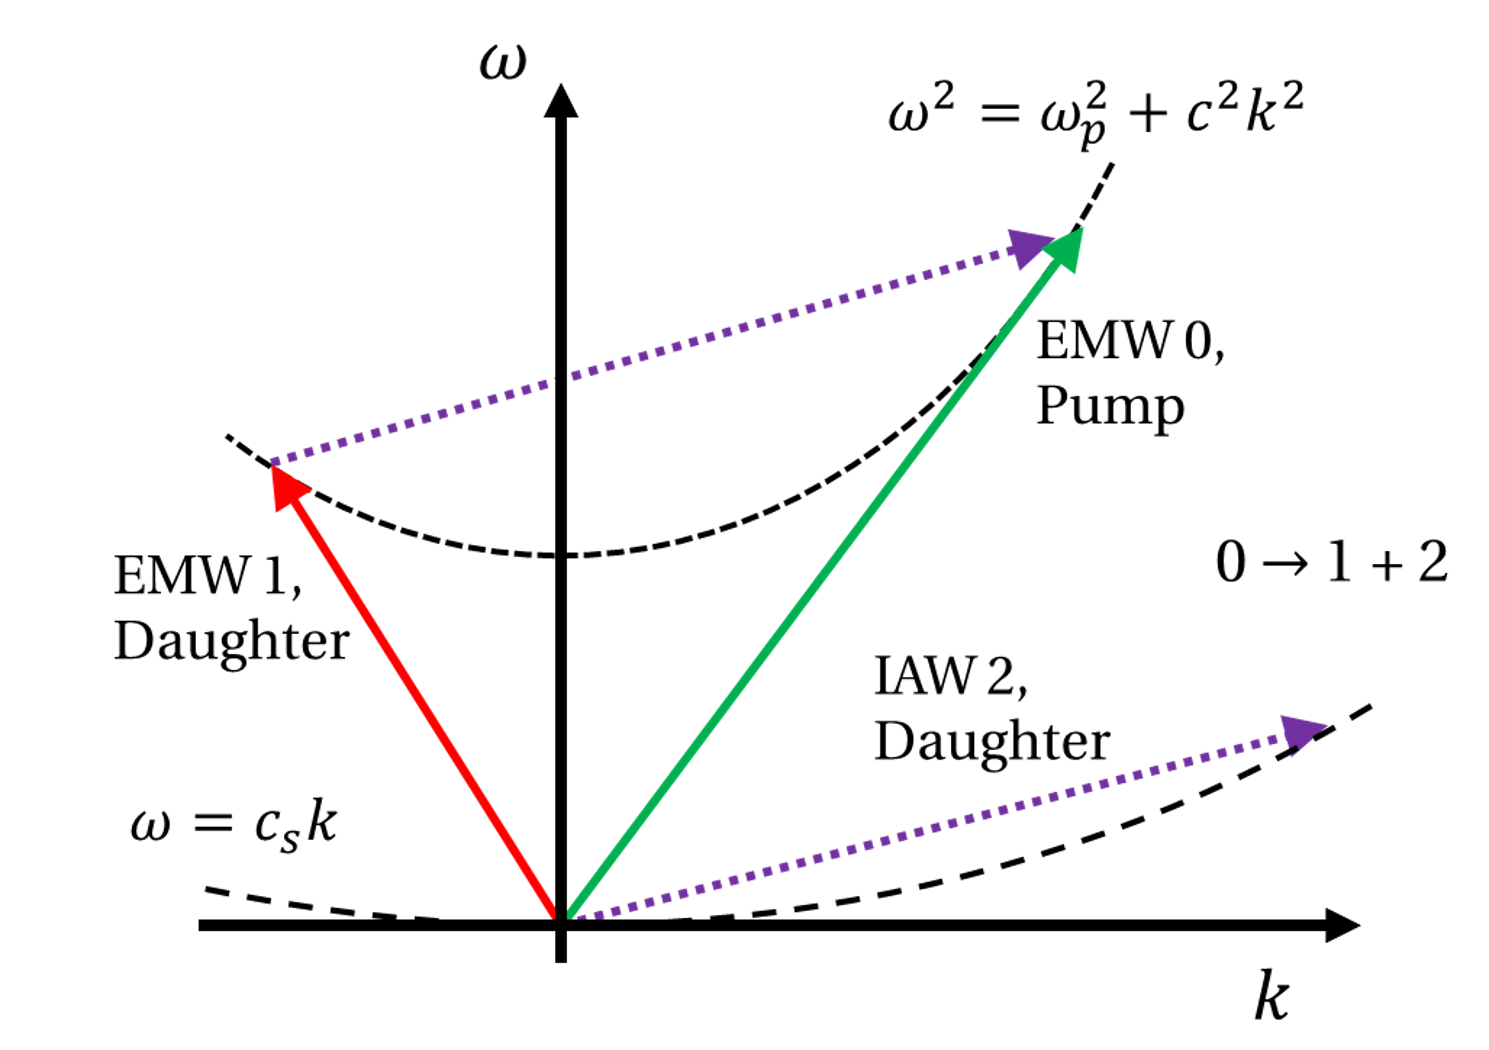
\includegraphics[width=0.6\linewidth]{Theory/Images/LPI_conservation_disprel.png}
    \centering
    \caption{The frequency and wave number matching conditions for \ac{LPIs}, whereby a pump \ac{EMW}, labelled 0, loses energy to two daughter waves.
        Here the daughter waves are another \ac{EMW} with lower frequency ($\omega_1<\omega_0$) and an \ac{IAW}, which are labelled 1 and 2, respectively.
        \ac{EMW}$\rightarrow$\ac{EMW}$+$\ac{IAW} identifies the process as \ac{CBET} or \ac{SBS}.
    }%
    \label{fig:theory_LPI_disprel}
\end{figure}

The frequency and wave number matching conditions for a resonant excitation can be expressed in the form,
\begin{align}
    \label{eq:theory_omega_match}
    \omega_2 = \omega_0 - \omega_1,\\
    \label{eq:theory_k_match}
    \vec{k}_2 = \vec{k}_0 - \vec{k_1},
\end{align}
where $\omega_2$ and $\vec{k}_2$ match the dispersion relation for either an \ac{EPW} or \ac{IAW}.
Wave `0' is often referred to as the `pump' wave and the other waves are known as the `daughter' waves.
Eqs.~\ref{eq:theory_omega_match} and~\ref{eq:theory_k_match} can heuristically be thought of as conservation of wave quanta energy and momentum, respectively.
This is seen more clearly by multiplying both sides by $\hbar$ and noting that the energy and momentum of a wave quanta are $\hbar\omega$ and $\hbar k$, respectively.
This conservation is illustrated in Fig.~\ref{fig:theory_LPI_disprel}, which plots the dispersion relations for \ac{CBET} or \ac{SBS}, whereby a pump \ac{EMW} loses energy to a daughter \ac{EMW} and \ac{IAW}.

%################################################################################
%################################################################################
\subsection{Cross-Beam Energy Transfer}%
\label{sec:theory_CBET}

\begin{figure}[t!]
    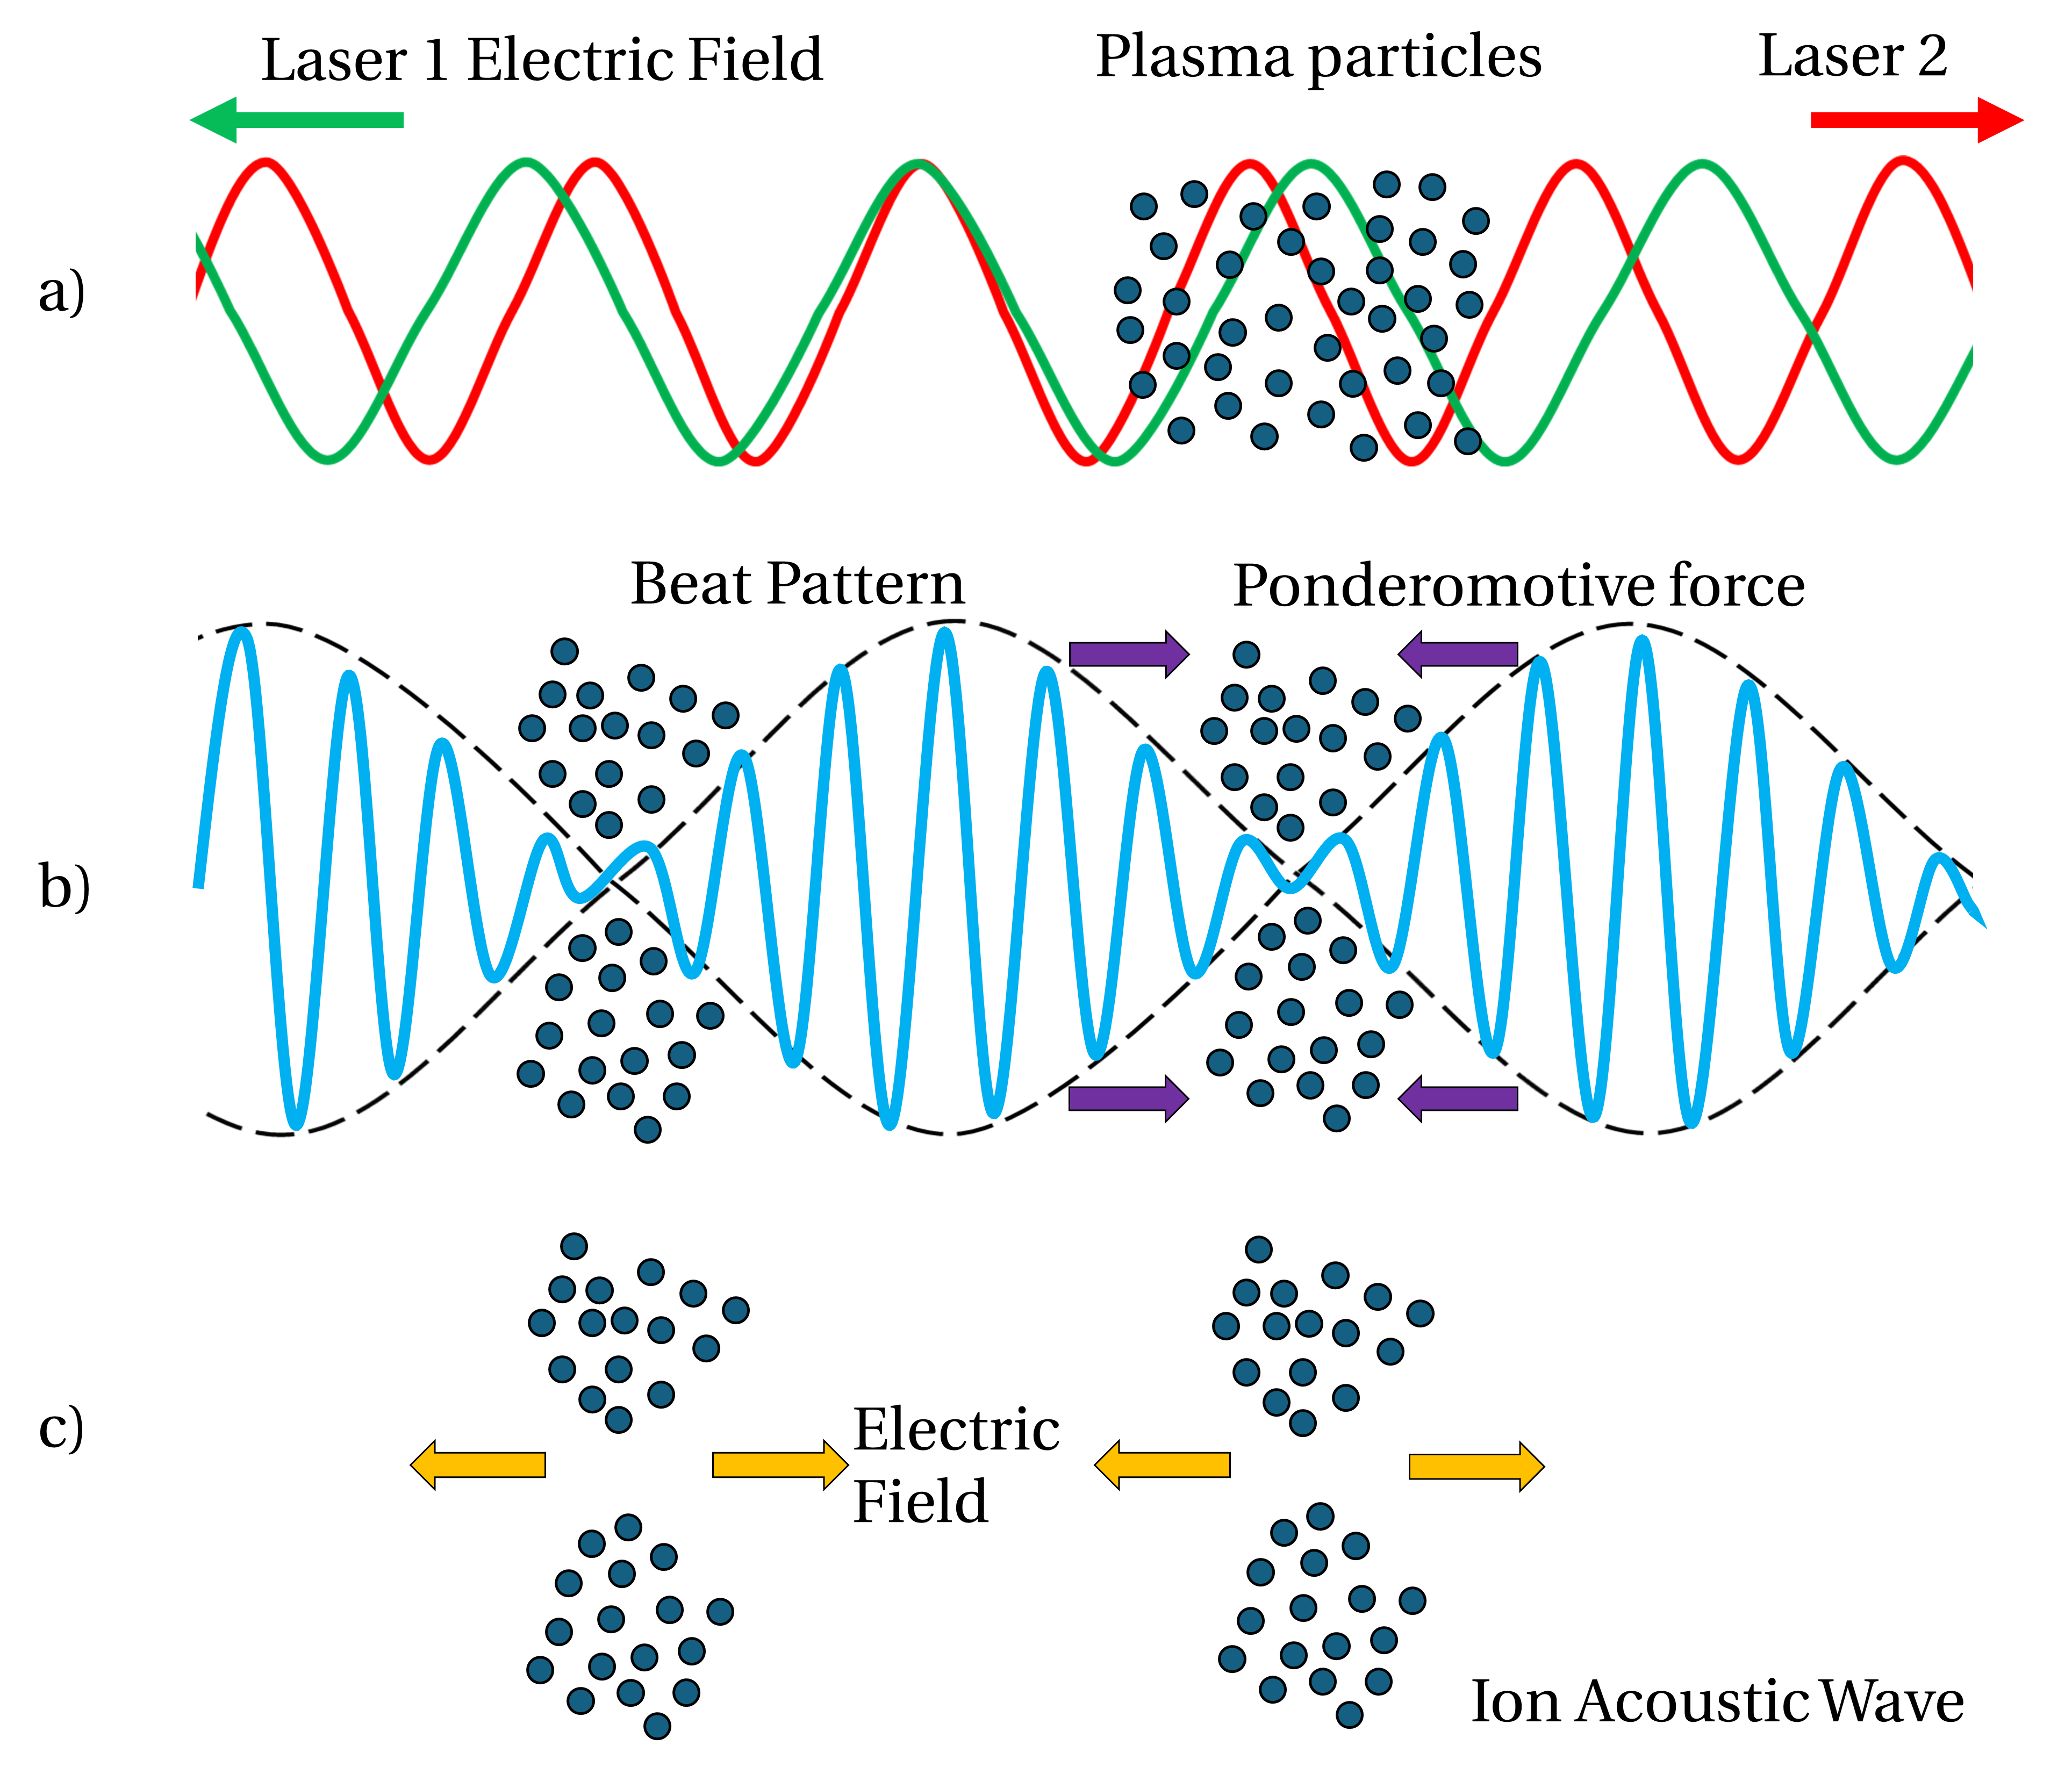
\includegraphics[width=0.8\linewidth]{Theory/Images/CBET_mechanism.png}
    \centering
    \caption{A 1-D Illustration of the mechanism by which \ac{CBET} grows.
    Panel a) plots the incident electric fields from two lasers, overlapping in a plasma background.
    This creates a beat pattern which ponderomotively pushes charges within the plasma to regions where the beat envelope is small, as is shown in panel b).
    If the spatial and temporal frequency of the beat oscillation matches the \ac{IAW} dispersion relation, then an \ac{IAW} grows, which is shown in panel c).
    The density modulation from the \ac{IAW} acts as a grating which transfers energy from one beam to the other.
    }%
    \label{fig:theory_CBET_mechanism}
\end{figure}

As stated, \ac{CBET} is one of the \ac{LPIs}, which involves the decay of an \ac{EMW} into another \ac{EMW} and an \ac{IAW}.
This is almost the same as \ac{SBS}, but distinct.
For \ac{SBS}, the daughter \ac{EMW} wave occurs due to light scattering from the plasma, and therefore grows from noise.
The scattered light wave is low amplitude, therefore its field can be amplified manyfold via the process.
In \ac{CBET} however, the daughter \ac{EMW} is another laser beam, \textit{i.e.} two laser beams cross leading to a beat pattern and subsequent energy exchange from one beam to another.
This procedure is illustrated in Fig.~\ref{fig:theory_CBET_mechanism}
Both light waves are relatively large in field amplitude and therefore a significant amount of energy can be transferred, even when the waves do not quite resonantly drive an \ac{IAW}~\cite{michel_introduction_2023}.

A fluid description of the plasma may be used as a useful starting point to introduce the key physics of \ac{CBET} and obtain a rate of energy transfer between the light waves, known as the gain.
A kinetic plasma description is often required to accurately model the interaction, especially when occurring in multi-species plasmas~\cite{williams_frequency_1995}.
While not provided here, the kinetic gain (derived in, for example, Ref.~\cite{michel_saturation_2013}) is presented in Sec.~\ref{sec:SOLAS_ray_power_change}, along with a description of its benefits over the fluid gain.
The fluid gain derivation was first calculated in Ref.~\cite{randall_theory_1981}. 

The system of equations to solve to calculate the gain rate of \ac{CBET} may be written as,
\begin{align}
    \label{eq:theory_CBET_interaction1}
    (\partial_t^2 + \omega_p^2 - c^2\nabla^2)\vec{a}_0 &= -\omega_p^2\frac{\delta n_e}{n_{e}}\vec{a}_1,\\
    \label{eq:theory_CBET_interaction2}
    (\partial_t^2 + \omega_p^2 - c^2\nabla^2)\vec{a}_1 &= -\omega_p^2\frac{\delta n_e}{n_{e}}\vec{a}_0,\\
    \label{eq:theory_CBET_interaction3}
    \left[ \left( \partial_t + \nu + \vec{u}.\nabla \right)^2 - c_s^2\nabla^2 \right]\frac{\delta n_e}{n_{e}} &= \frac{Z m_e c^2}{m_i}\nabla^2 (\vec{a}_0 . \vec{a}_1).
\end{align}
In Eqs.~\ref{eq:theory_CBET_interaction1} and~\ref{eq:theory_CBET_interaction2}, $\vec{a}_i$ are the normalised vector potentials of the light waves, which undergo an interaction proportional to the density modulation generated by an \ac{IAW}, $\delta n_e/n_{e}$.
These equations describe the general coupling of two light waves via an \ac{IAW}.
Eq.~\ref{eq:theory_CBET_interaction3} is the driven wave equation for the \ac{IAW} in a plasma with flow velocity $\vec{u}$ and ionisation $Z$, which experiences damping, $\nu$.
Much more detail on the derivation and solution of this system of equations is provided in Ref.~\cite{michel_introduction_2023}, however, a final amplification rate is obtained,
\begin{align}
    \label{eq:theory_CBET_linear_gain}
    \gamma_{01} &= \frac{n_e e}{4 m_e c \omega_0} \frac{1}{T_e \left( 1 + 3 T_i / Z T_e \right)} \frac{R(\eta_{01})}{\nu}, \\
    R(\eta_{01}) &= \frac{ (\nu/\omega_{s})^2 \eta_{01} } { (\eta_{01}^2 - 1)^2 + (\nu/\omega_s)^2 \eta_{01}^2 }, \\
    \label{eq:theory_resonace_param_fluid}
    \eta_{01} &= \frac{ \omega_\Delta - \vec{k}_\Delta.\vec{u} }{\omega_s},
\end{align}
where $T_e$ and $T_i$ are the electron and ion temperatures in $\text{eV}$ respectively and $\omega_s = |\vec{k}_\Delta|c_s$ is the \ac{IAW} frequency.
The gain, $\gamma_{01}$ describes the spatial amplification rate per unit path length of beam 0 interacting with beam 1, such that $|a_i|^2\sim |a_{i0}|^2\exp{(\gamma_{ij}|a_{j0}|^2 \text{d}\tau)}$.
The key assumptions in the derivation of Eq.~\ref{eq:theory_CBET_linear_gain} include assuming a linear plasma response, such that the effect of the ponderomotive force can be treated perturbatively.
This proves to be a good assumption for the intensities used in direct-drive \ac{ICF}, which are specifically limited to avoid the non-linear regime where \ac{LPIs} can dominate.
Another assumption is that the plasma and pump field are homogeneous over the interaction length.
For implementation in a ray-tracing code, this is a good assumption because the gain is applied over ray steps, which are by necessity small compared to gradient length scales of the plasma.
Additionally, the interaction is assumed to be in a steady state.
This is satisfied for direct-drive \ac{ICF} on the \textsc{Omega} facility because the \ac{CBET} saturation timescale of $\sim10\ \text{ps}$ is shorter than the hydrodynamic time scale of $\sim100\ \text{ps}$.
A final assumption was used, that the fields were had parallel polarisation, which shall be discussed in Sec.~\ref{sec:theory_cbet_polarisation}. 

\begin{figure}[t!]
    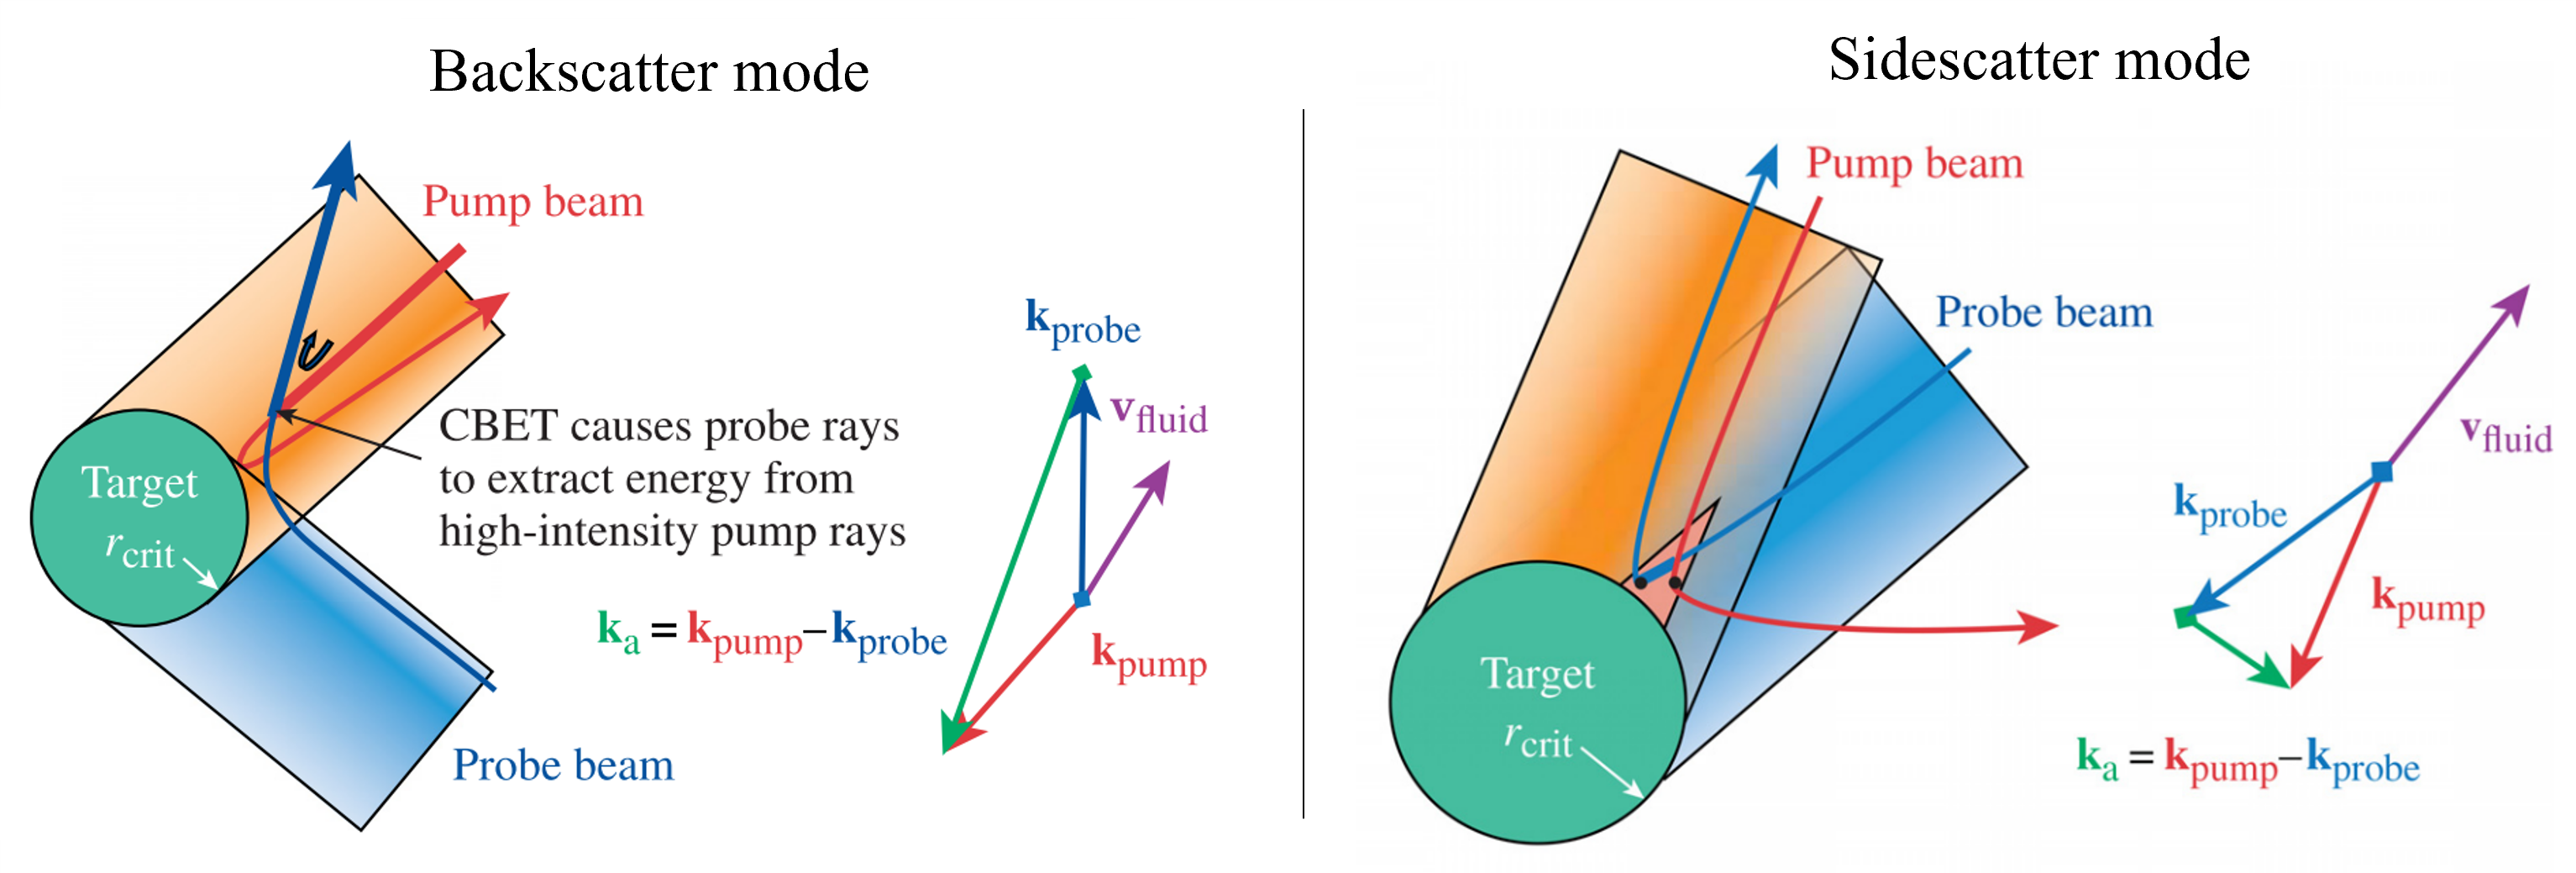
\includegraphics[width=\linewidth]{Theory/Images/CBET_modes.png}
    \centering
    \caption{The two \ac{CBET} modes which are identified from the fluid \ac{CBET} gain in Eq.~\ref{eq:theory_CBET_linear_gain}, in the context of direct-drive \ac{ICF}.
    The backscatter mode (left) dominates for direct-drive \ac{ICF}.
    In this regime, the light waves have approximately equal frequencies and therefore the required frequency difference in the plasma frame to excite an \ac{IAW} is a result of the Doppler shift.
    In the sidescatter mode (right) which is employed in indirect-drive to tune symmetry~\cite{michel_tuning_2009}, the flow is orthogonal to the wave vector and therefore \ac{CBET} only occurs due to a frequency difference between the waves.
    This figure has been reproduced with permission from Ref.~\cite{marozas_wavelengthdetuning_2018}.
    }%
    \label{fig:theory_CBET_modes}
\end{figure}

Maximal scattering occurs when the resonance parameter, $\eta_{01}=1$.
Eq.~\ref{eq:theory_resonace_param_fluid} therefore identifies two distinct regimes when a resonance can be achieved, which are shown in Fig.~\ref{fig:theory_CBET_modes}.
In a stationary plasma (or when $\vec{k}_\Delta \perp \vec{u}$), scattering can only occur when the beams have a frequency difference, which is known as the sidescatter mode.
Alternatively, if the beams have equal frequency, the plasma flow term in the numerator of Eq.~\ref{eq:theory_resonace_param_fluid} ($\vec{k}_\Delta.\vec{u}$), acts to Doppler shift the frequencies of the laser beams in the frame of the plasma.
This results in a frequency difference which can drive an \ac{IAW} if $|\vec{u}|\approx c_s$.
Direct-drive coronal plasma flow is supersonic and therefore backscatter \ac{CBET} occurs close to the Mach-1 surface.
The plasma flow in the corona is approximately radially outward, and thus the Doppler shift acts to increase the frequency of the radially inward travelling beam in the plasma frame.
From the energy conservation condition in Eq.~\ref{eq:theory_omega_match}, energy is therefore depleted from the inbound laser beam and transferred to the outbound beam.
The Mach-1 surface is significantly separated from the region close to critical, where \ac{Inv-Brem} deposition is important and therefore energy is effectively reflected in direct-drive implosions by backscatter \ac{CBET} before it is deposited within the plasma.
Although all lasers on the \textsc{Omega} laser facility have the same frequency, the frequency shift term from Eq.~\ref{eq:theory_doppler}, means that lasers which have propagated through a different plasma profile have slightly different frequencies.
Although small, this shift is often of the order of the numerator terms in Eq.~\ref{eq:theory_resonace_param_fluid} and thus must be included when modelling direct-drive \ac{CBET}.\footnote{Typically, the frequency difference for light which has propagated through a steady state direct-drive corona is on the order of $\Delta\omega/\omega\sim\mathcal{O}(0.1\%)$.}
For indirect-drive implosions, the \ac{LEH} where the lasers cross does not have significant plasma flow.
Therefore, in order to tune the symmetry of capsules implosions with \ac{CBET}, the sidescatter mechanism is utilised, by introducing a finite frequency difference between the inner and outer cones of beams.
The frequency difference is experimentally tuned to obtain a round implosion morphology~\cite{michel_tuning_2009}.

%##########################################################
\subsubsection{Effect of Polarisation}%
\label{sec:theory_cbet_polarisation}

\ac{CBET} is affected by the polarisation of the light waves which seed it.
Only the parallel polarisation components of the waves create the ponderomotive beat field which sets up the density modulation.
In the case of mixed polarisation, the gain rate can simply be reduced by multiplying by a random polarisation factor, which is provided in Eq.~\ref{eq:polarisation_smoothing}.
Polarisation smoothing optics are typically employed on direct-drive facilities which create a mixed polarisation beam, as described in Sec.~\ref{sec:intro_direct_phys}.
In reality, however, the \ac{DPRs} on \textsc{Omega} do not actually create a single, mixed polarisation laser spot, but two slightly offset sub-beams on the target.
\ac{CBET} models which track polarisation or rays have been developed, which account for the true polarisation angle between two beams~\cite{edgell_nonuniform_2021,colaitis_3d_2022,colaitis_3d_2023,colaitis_3d_2023a}.
These models have demonstrated that polarised \ac{CBET} on \textsc{Omega} creates a mode-1 which is always in the same direction.
This persistent mode-1 was experimentally observed from neutron time of flight diagnostics before its origin was understood~\cite{mannion_mitigation_2021}.

%##########################################################
\subsubsection{Langdon Effect on CBET}%
\label{sec:theory_cbet_langdon}

As was described in Sec.~\ref{sec:theory_in_brem}, \ac{Inv-Brem} preferentially heats the colder electron population, leading to a super-Gaussian electron distribution function.
A non-Maxwellian distribution function has an altered susceptibility to the \ac{IAW}~\cite{afeyan_kinetic_1998}, and therefore \ac{Inv-Brem} heated plasmas have a modified resonance condition for \ac{CBET}.
Dedicated experiments have been performed which used Thompson scattering to measure the electron distribution function of an \ac{Inv-Brem} heated, gas jet plasma  in order to study how \ac{CBET} is modified~\cite{turnbull_impact_2020}.
These experiments demonstrated that the \ac{CBET} gain was systematically reduced by an altered dispersion relation,
\begin{equation}
    \omega = k c_s \left[ \frac{3 \Gamma^2(3/m)}{\Gamma(1/m)\Gamma(5/m)} \right]^{1/2},
\end{equation}
where $\Gamma$ is the Gamma function and,
\begin{equation}
    m(\alpha) = 2 + \frac{3}{1 + 1.66/\alpha^{0.724}},
\end{equation}
and $\alpha$ is defined in Eq.~\ref{eq:theory_alpha_langdon}.
This is a small effect in direct-drive experiments on \textsc{Omega} due to the relatively low amplitude overlapped field strengths in a direct-drive geometry~\cite{colaitis_inverse_2021}.
However, reduction of the gain via Langdon disturbing the electron distribution function could be one possible explanation for why \ac{CBET} calculations on the \ac{NIF} are not predictive and require an artificial clamp on the \ac{IAW} amplitude~\cite{michel_stochastic_2012,kritcher_energy_2018}.

%################################################################################
%################################################################################
\subsection{Mitigation of Cross-Beam Energy Transfer}%
\label{sec:theory_lpi_mitigation}

\ac{LPIs} are significantly detrimental to \ac{ICF} experiments.
For example, direct-drive experiments on \textsc{Omega} experience a 50\% deposition reduction instantaneously, which particularly occurs late in the implosion at peak incident power~\cite{colaitis_inverse_2021}.
This severely limits the ablation and therefore stagnation pressures which can be achieved.
Mitigation of \ac{LPIs} and particularly \ac{CBET} is an active area of investigation related to direct-drive \ac{ICF} and there are several distinct approaches which have been explored.

For \ac{LPIs} to occur, there must be a spatial, temporal and spectral matching between waves.
Spatially and temporally, the light waves must be in the same place and at the same time to create the ponderomotive beat pattern that excites plasma waves.
The spatial coherence can be reduced by changing the widths of the beams involved in the interaction.
For example, a narrower beam profile can be used for direct-drive implosions, which leads to less refracted light travelling away from the target to act as a seed for \ac{CBET} when crossing other beams~\cite{froula_increasing_2012}.
This is explored in more detail in Chap.~\ref{chap:RbRt}.
Although \ac{CBET} scattering can be significantly reduced by taking this approach, which greatly increases energy coupling, the performance of the implosion becomes limited by the lack of symmetry due to large beam-modes.
An improvement to this approach is to dynamically alter the size of the beams that drive the implosion to match the shrinking critical surface, which is known as zooming~\cite{froula_mitigation_2013}.
If the beam width shrinks to match the critical radius of the target, then beam-mode growth is not large, which increases energy coupling without loss of stagnation state symmetry~\cite{igumenshchev_laserbeam_2013}.
Zooming does require specialised laser optics which are not present on the \ac{NIF} or the \textsc{Omega} laser system however~\cite{kehne_implementation_2013}, and therefore it is not a mitigation strategy that can be employed on current direct-drive implosion experiments.
Temporal coherence can be broken by modulating the laser pulses in time with a high frequency.
These pulse types are known as STUD pulses and act to disrupt the growth of \ac{LPIs}~\cite{afeyan_optimal_2013}.

The majority of current mitigation research focuses on disrupting the spectral coherence required for \ac{LPIs} to grow.
This approach suggests either using laser systems with multiple discrete wavelengths~\cite{edgell_mitigation_2017,marozas_first_2018,marozas_wavelengthdetuning_2018}, or employing broadband lasers~\cite{bates_mitigation_2018,bates_suppressing_2023}, to break the spectral coherence required for \ac{CBET} and other \ac{LPIs}.
Particularly, bandwidth is thought to be the most promising technology for implementation on a future laser system, as it is possible to almost entirely eliminate \ac{CBET} and \ac{SBS} with sufficient bandwidth.
Specifically for \ac{CBET}, with sufficient bandwidth, power transfer can occur `backwards' in the backscatter mode, whereby energy is also transferred from the outgoing light to the incoming light, leading to almost no net energy exchange~\cite{seaton_crossbeam_2022}.
Bandwidth on the order of $\Delta\omega/\langle\omega\rangle\sim1\%$ is found from ray-based modelling to be sufficient to effectively mitigate \ac{CBET}~\cite{colaitis_exploration_2023,follett_raybased_2023}, which is in agreement with wave-based~\cite{bates_suppressing_2023} and kinetic~\cite{seaton_crossbeam_2022} modelling.
Eliminating \ac{CBET} and other \ac{LPIs} would also open up the design space for new implosions, because peak intensities would no longer be limited to $\sim10^{15}\ \text{W/cm}^2$.
This would increase the viability of, for example, shock ignition designs, with high intensity ignitor pulses late in the implosion~\cite{betti_shock_2007,perkins_shock_2009,scott_shockaugmented_2022}.
A single broadband beam ($\Delta\omega/\langle\omega\rangle>1\%$), known as the \textsc{Flux} laser is currently under development on the \textsc{Omega} laser facility, to explore the effectiveness of bandwidth to mitigate \ac{CBET}~\cite{deeney_advances_2022}.
Bandwidth has the additional benefit that it would reduce laser imprint when passed through \ac{SSD} optics.
